\documentclass{SBCbookchapter}
\usepackage[T1]{fontenc}
\usepackage[utf8]{inputenc}
\renewcommand*\ttdefault{txtt}

\usepackage[brazilian, american]{babel}

% \usepackage{array}
% \usepackage{ifpdf}
% \usepackage{subfigure}
% \usepackage{color}
% \usepackage{framed}
% \usepackage{hyperref}

\usepackage{graphicx}
\usepackage{cite}
\usepackage{url}
\usepackage{comment}

\usepackage{verbatimbox}
\usepackage{minted}
\newminted{verilog}{linenos}

% \usepackage{tikz}
% \usetikzlibrary{shapes.callouts}
% \usetikzlibrary{shadows}

\newcommand{\ssf}[1]{\texttt{\small{}#1}}
\newcommand{\sssf}[1]{\texttt{\scriptsize{}#1}}

\newcommand{\figstr}{figura}
\newcommand{\Figstr}{Figura}
\newcommand{\tabstr}{tabela}
\newcommand{\Tabstr}{Tabela}
\newcommand{\secstr}{seção}
\newcommand{\Secstr}{Seção}

\pagestyle{plain}
\pagenumbering{arabic}

\hyphenation{Net-FPGA}

\author{\vspace{2mm}Pablo Goulart, Ítalo Cunha, Marcos A. M. Vieira (UFMG)\newline
Cesar Marcondes, Ricardo Menotti (UFSCar)}

\title{NetFPGA: Processamento de Pacotes em \emph{Hardware}}

\begin{document}

\maketitle

\selectlanguage{american}

\begin{abstract}

The NetFPGA platform allows general-purpose network packet processing in hardware. NetFPGAs can be used to develop research prototypes and deploy new network functionality. This tutorial will present NetFPGA's hardware architecture, its programming interface, and possible applications. We will demonstrate all steps in the implementation and deployment of a hardware firewall to filter packets depending on the TCP destination port.  The concepts covered in this tutorial will help researchers and programmers use the NetFPGA with any of its available modules as well as develop new hardware packet processing modules.

\end{abstract}

\selectlanguage{brazilian}

\begin{resumo}

A plataforma NetFPGA permite processamento genérico de pacotes de rede
em \emph{hardware}. A NetFPGA pode ser utilizada para desenvolvimento de
protótipos de pesquisa bem como implantação de novas funcionalidades.
Este minicurso apresentará a arquitetura de hardware da NetFPGA, a
interface de programação e possíveis aplicações da NetFPGA. Iremos
demonstrar passo-a-passo a implementação de um \emph{firewall} para
filtragem de pacotes em hardware em função da porta de destino do
protocolo TCP.  Os conceitos do minicurso irão permitir pesquisadores e
programadores utilizarem a NetFPGA com módulos existentes, bem como
desenvolverem novos módulos para processamento de pacotes em hardware.

\end{resumo}

% \printglossary[type=\acronymtype]
% \renewcommand*{\glspostdescription}{}
% Delete the trailing point if using package glossaries with
% nonumberlist as arguments
%\printglossary[style=super,nonumberlist,type=\acronymtype,title=Acrônimos]

\newpage
\section{Introdução}

Comutadores (\emph{switches}) e roteadores (\emph{routers}) atuais
suportam uma quantidade limitada de arquiteturas e protocolos de
rede.  Mesmo para as arquiteturas e protocolos suportados,
comutadores e roteadores permitem processamento limitado dos
pacotes, como decremento do TTL, verificação do \emph{checksum},
balanceamento de carga e descarte.  Esta falta de flexibilidade
dificulta a avaliação e implantação de mecanismos como
OpenSketch~\cite{yu13opensketch}, de protocolos alternativos como
Free-riding Multicast~\cite{ratnasamy06multicast} e de novas
arquiteturas como XIA~\cite{han12xia}, CCN~\cite{jacobson09content},
ou SDN~\cite{casado09ethane}.  O caminho padrão para avaliação e
implantação dessas soluções seria desenvolver novas placas de rede e
processadores de pacotes específicos em \emph{hardware} (ASICs), o
que é economicamente inviável.

A NetFPGA é uma plataforma aberta que combina um FPGA
(\emph{field-programmable gate array}, ou arranjo de portas
programável em campo) memória (SRAM e DRAM) e processadores de
sinais numa placa com quatro portas Ethernet de 1\,Gbps ou 10\,Gbps.
Desenvolvedores podem programar o FPGA e utilizar a memória para
implementar novos mecanismos, protocolos e arquiteturas.  A NetFPGA
permite modificação dos pacotes em trânsito, controle total sobre o
encaminhamento e manutenção de estado.

A NetFPGA é particularmente útil como uma alternativa de
\emph{hardware} flexível e de baixo custo para avaliação de
protótipos de pesquisa.  NetFPGAs já foram utilizadas em vários
projetos de pesquisa (e.g.,~\cite{yu13opensketch,
Naous:2008:IOS:1477942.1477944, ghani10secure, thinh12fpga,
antichi12open, lombardo12netfpga}).  Comparada com a abordagem de
implementar soluções em \emph{software}, a NetFPGA garante
processamento e encaminhamento na taxa de transmissão das interfaces
(sem sacrificar banda), baixa latência e não onera a CPU do
computador.

% A plataforma NetFPGA permite processamento genérico de pacotes de
% rede em hardware.  A NetFPGA pode ser utilizada para
% desenvolvimento de protótipos de pesquisa bem como implantação de
% novas funcionalidades.

Neste texto, introduziremos o leitor à NetFPGA. Na
\secstr~\ref{sec:example} iremos demonstrar nosso \emph{firewall} em
funcionamento do ponto de vista do usuário e descreveremos como
configurar o ambiente de desenvolvimento da NetFPGA.  Na
\secstr~\ref{sec:arch} iremos apresentar as arquiteturas de
\emph{hardware} e \emph{software} da NetFPGA, dando uma visão geral
das funcionalidades e do desenvolvimento na NetFPGA.  Na
\secstr~\ref{sec:impl} iremos demonstrar passo-a-passo a criação de
um novo módulo na NetFPGA.  Usaremos como exemplo um \emph{firewall}
para filtragem de pacotes em \emph{hardware} em função da porta de
destino do protocolo TCP.  Nosso \emph{firewall} é um exemplo
didático que cobre a maior parte dos conceitos necessários para
desenvolvimento de um novo projeto, como utilização de memória bem
como processamento e modificação de pacotes.  Por fim, na
\secstr~\ref{sec:related} iremos discutir outros projetos utilizando
a NetFPGA.  Acreditamos que os conceitos do minicurso irão permitir
pesquisadores e programadores utilizarem a NetFPGA com módulos
existentes bem como desenvolverem novos módulos para processamento
de pacotes em \emph{hardware}.



\newpage
\section{Visão do usuário da aplicação exemplo: um \emph{firewall} na NetFPGA}
\label{sec:example}

Nesta seção iremos explicar como preparar o ambiente de
desenvolvimento para NetFPGA e iremos exemplificar a aplicação
exemplo que iremos implementar, um \emph{firewall}.  Nosso
\emph{firewall} é detectado pelo sistema operacional como uma
interface de rede Ethernet padrão.  Esta interface pode ser
configurada com um endereço IP e transmitir pacotes de rede
normalmente.  Porém, podemos também configurar a interface do
\emph{firewall} para filtrar pacotes TCP destinados a um conjunto de
portas que queremos bloquear.  Nosso \emph{firewall} faz o
processamento e filtragem dos pacotes TCP na NetFPGA, sem consumir
capacidade de processamento no computador hospedeiro.  As portas que
queremos bloquear podem ser configuradas dinamicamente por programas
de espaço do usuário, ou seja, sem a necessidade de reconfiguração
do FPGA.

A maioria dos comandos mostrados nesta seção devem ser digitados no
terminal do Linux como superusuário (\emph{root}).  Quando se tratar
de comandos a serem incluídos ou modificados em arquivos o caminho
completo destes será fornecido.

\subsection{Preparação do ambiente de desenvolvimento}

Nesta seção apresentamos o ambiente de desenvolvimento da NetFPGA.
Mostramos como configurar o ambiente de desenvolvimento num
computador e utilizamos nosso \emph{firewall} para demonstrar
passo-a-passo a utilização do ambiente de desenvolvimento.

As instruções são baseadas na documentação oficial da
NetFPGA,\footnote{\sssf{https://github.com/NetFPGA/netfpga/wiki/Guide}}
com algumas adições para tratar possíveis dificuldades durante a
configuração do ambiente.  O nosso ambiente de desenvolvimento é
baseado no Fedora Linux 13
(32-bits)\footnote{\sssf{http://archives.fedoraproject.org/pub/archive/fedora/linux/releases/13/Live}}
e no Xilinx ISE
10.1,\footnote{\sssf{http://www.xilinx.com/support/download/index.html/content/xilinx/en/downloadNav/design-tools/archive.html}}
que são recomendados para uso com a NetFPGA; mas é possível utilizar
outras distribuições e versões da ferramenta.  Fique atento ao
consultar a documentação oficial, pois na documentação oficial
encontramos instruções relativas a diferentes versões da NetFPGA; em
nosso curso usamos a NetFPGA 1G.

A forma mais prática de se obter um ambiente de simulação é fazendo
o download de uma máquina virtual (VM) pré-configurada. Nas
instruções a seguir apresentamos como configurar uma máquina
virtual.  As instruções para instalação de uma máquina virtual
também se aplicam para a instalação e configuração de uma máquina
real, inclusive com uma placa (\emph{hardware}) NetFPGA.  Neste
tutorial utilizamos o
VirtualBox\footnote{\sssf{https://www.virtualbox.org}} para
exemplificar a configuração de uma máquina virtual pois este está
disponível para Windows, Linux e Mac.  Se quiser configurar uma
máquina real, grave a imagem do Fedora em um CD ou DVD para
posterior instalação.

\subsubsection{Criação de uma máquina virtual}

Nesta seção descrevemos como criar uma máquina virtual no VirtualBox
para instalar o ambiente de desenvolvimento.  Se você deseja
instalar uma máquina real inicie o computador a partir do CD ou DVD
do Fedora e siga para a \secstr~\ref{ssec:linux}.

% \begin{figure}[H]
% \centering
% 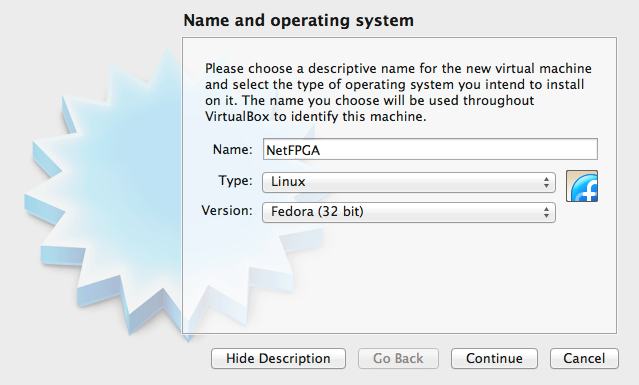
\includegraphics[scale=0.5]{figures/vm/vm1}
% \caption{Nome tipo e versão do sistema a ser instalado}
% \label{fig:vm.sys}
% \end{figure}

Instale o VirtualBox em seu sistema, execute-o e abra o tutorial
para criação de uma nova máquina virtual utilizando o menu
\emph{Machine $\rightarrow$ New}.  Escolha um nome para sua máquina
virtual (por exemplo, ``NetFPGA''), configure o tipo de máquina
virtual para ``Linux'' e a versão para ``Fedora (32 bit).''  No
passo seguinte, selecione a quantidade de memória desejada para a
máquina virtual.  Sugerimos pelo menos 3\,GiB para executar o Xilinx
ISE, mas você pode aumentar este valor se tiver memória disponível
no sistema hospedeiro.  Na próxima etapa, selecione a segunda opção
para criar um novo disco virtual (\emph{Create a virtual hard drive
now}).  Sugerimos o formato padrão para o disco virtual (VDI).
Sugerimos também utilização de alocação dinâmica de espaço para que
o disco virtual ocupe apenas o espaço necessário (\emph{Dynamically
allocated}).  Para finalizar esta etapa, indique o mesmo nome da
máquina virtual para facilitar a identificação do disco (por
exemplo, ``NetFPGA'') e selecione seu tamanho máximo.  É recomendado
selecionar um espaço razoável para o disco (pelo menos 20\,GB).
Como só será alocado o espaço necessário, aumentar o tamanho máximo
não implica custo.

% \begin{figure}[H]
% \centering
% 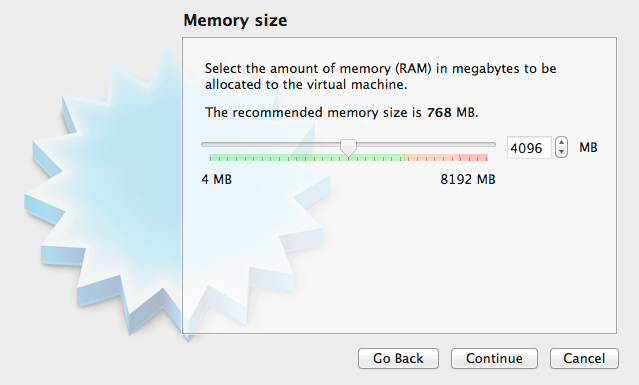
\includegraphics[scale=0.5]{figures/vm/vm2}
% \caption{Memória da máquina virtual}
% \label{fig:vm.mem}
% \end{figure}

% \begin{figure}[H]
% \centering
% 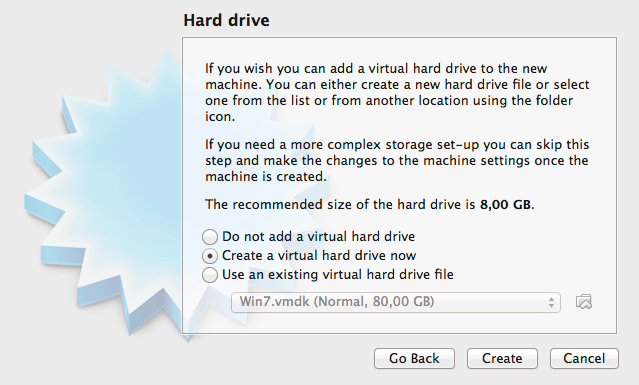
\includegraphics[scale=0.5]{figures/vm/vm3}
% \caption{Criar um novo disco virtual}
% \label{fig:vm.disk}
% \end{figure}

% \begin{figure}[H]
% \centering
% 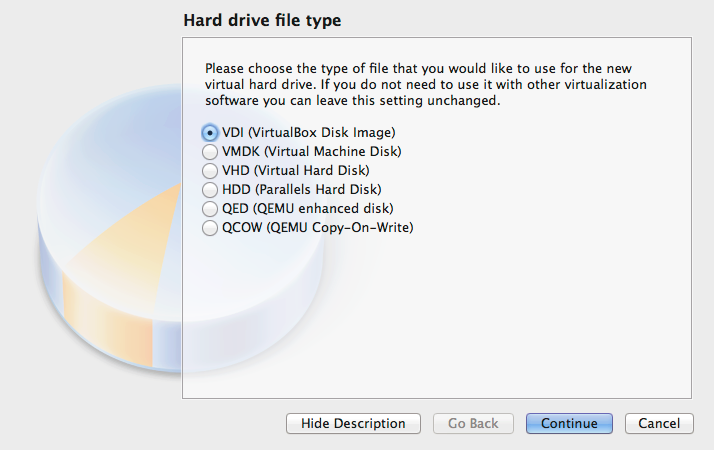
\includegraphics[scale=0.5]{figures/vm/vm4}
% \caption{Formato do disco virtual}
% \label{fig:vm.vdi}
% \end{figure}

% \begin{figure}[H]
% \centering
% 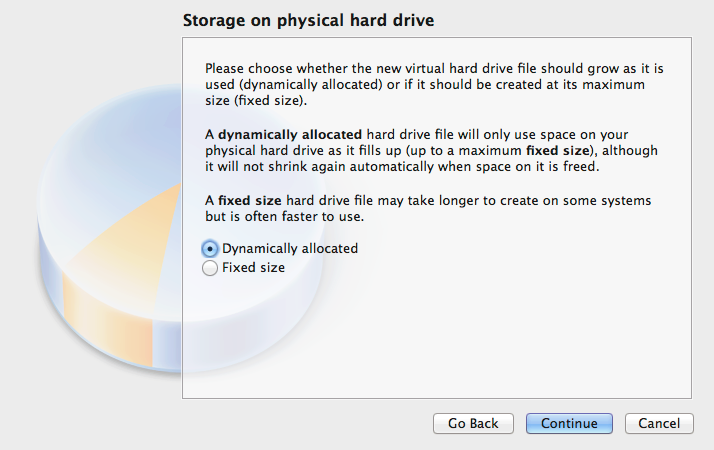
\includegraphics[scale=0.5]{figures/vm/vm5}
% \caption{Disco dinamicamente alocado}
% \label{fig:vm.dyn}
% \end{figure}

% \begin{figure}[H]
% \centering
% 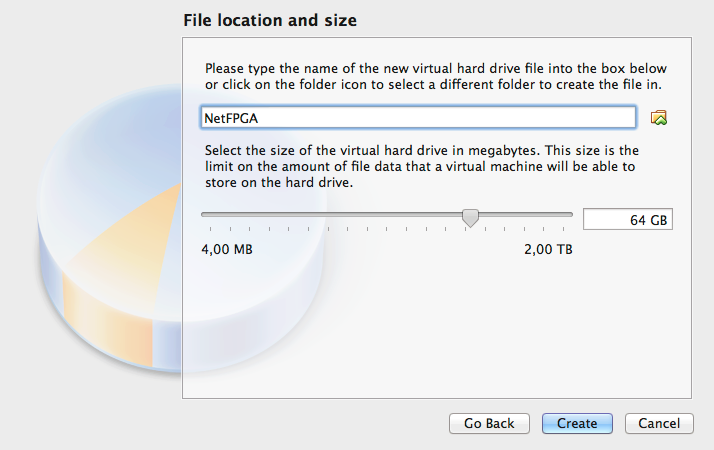
\includegraphics[scale=0.5]{figures/vm/vm6}
% \caption{Tamanho do disco virtual}
% \label{fig:vm.size}
% \end{figure}

% \begin{figure}[H]
% \centering
% 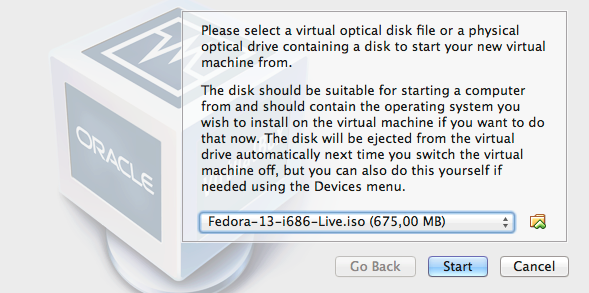
\includegraphics[scale=0.5]{figures/vm/vm7}
% \caption{Imagem para instalação do sistema}
% \label{fig:vm.cd}
% \end{figure}

Voltando à tela principal do VirtualBox, clique no botão
\emph{Start} para iniciar a máquina criada. Na primeira
inicialização o VirtualBox irá solicitar uma imagem de CD ou DVD de
instalação, indique o arquivo da imagem do Fedora 13. Os passos
seguintes são os mesmos, tanto para um sistema real quanto para a
máquina virtual.

\subsubsection{Instalação e configuração do sistema}
\label{ssec:linux}

% \begin{figure}[H]
% \centering
% 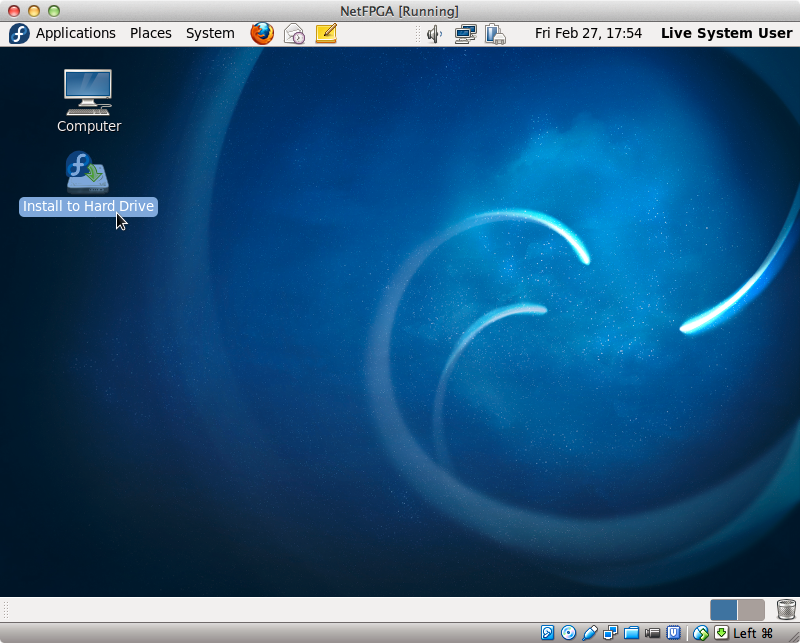
\includegraphics[scale=0.5]{figures/vm/vm8}
% \caption{Sistema inicializado a partir do CD/DVD Live}
% \label{fig:vm.live}
% \end{figure}

% \begin{figure}[!h]
% \centering
% 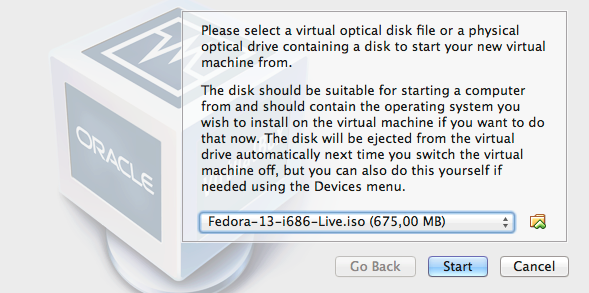
\includegraphics[scale=0.5]{figures/vm/vm7}
% \end{figure}

A inicialização a partir do CD ou DVD Live carrega o sistema para a
memória RAM, sem fazer qualquer alteração no disco. Após a
inicialização do sistema, selecione \emph{Install to hard drive}
para instalar o sistema no disco.  Siga os passos necessários para
selecionar o disco, determinar sua região e definir uma senha para o
superusuário (\emph{root}). Após finalizar a instalação, selecione o
comando de menu \emph{System $\rightarrow$ Shut Down} e reinicie o
computador (\emph{Restart}). Se estiver em uma máquina real, remova
o CD ou DVD da unidade. Se estiver em uma máquina virtual, desligue
o computador em vez de reiniciá-lo (\emph{Shut Down}), vá no
gerenciador de armazenamento (menu \emph{Settings $\rightarrow$
Storage}) e remova a imagem de CD ou DVD para iniciar a máquina
virtual a partir do disco virtual.

Após reiniciar o sistema é necessário informar mais algumas
configurações e criar uma conta de usuário. Para executar alguns dos
comandos usados neste minicurso é preciso ter acesso de superusuário
(\emph{root}), especialmente aqueles que fazem modificações no
sistema.  Por padrão, o Fedora não permite o \emph{login} como
\emph{root} no modo gráfico. Para contornar esta restrição é
possível usar o comando \ssf{su} que permite a um usuário comum
executar um \emph{shell} como \emph{root}. Se preferir modificar o
sistema para permitir o \emph{login} como \emph{root}, faça
\emph{login} na conta de usuário, acesse o diretório
\ssf{/etc/pam.d/} e edite os arquivos \ssf{gdm} e
\ssf{gdm-password}, comentando a seguinte linha em ambos:

\begin{verbnobox}[\small]
auth   required    pam_succeed_if.so user != root quiet
\end{verbnobox}

Os passos seguintes devem ser executados como \emph{root}, portanto
faça \emph{login} como \emph{root} ou use o comando \ssf{su} para
executar um \emph{shell} como \emph{root}.  A primeira modificação
necessária em nosso sistema é desabilitar o Security-Enhanced Linux
(SELinux). Para tal, edite o arquivo \ssf{/etc/selinux/config} e
mude a variável \ssf{SELINUX} para \ssf{disabled}.

A seguir, faremos a instalação de alguns pacotes necessários. Acesse
o diretório \ssf{/etc/yum.repos.d/} edite cada um dos arquivos com
extensão \ssf{.repo} trocando \ssf{https} das URLs por \ssf{http}.
Em seguida digite os seguintes comandos:

\begin{minted}{bash}
yum update
yum install gcc kernel-devel libnet-devel java-1.6.0-openjdk-devel
            python-argparse scapy wget iverilog gtkwave hping3 iperf
\end{minted}

Recomendamos também a instalação dos \emph{drivers} para o
VirtualBox através do menu \emph{Devices $\rightarrow$ Insert Guest
Additions CD Image}.

\subsubsection{Instalação das ferramentas}
\label{ssec:tools}

A seguir vamos configurar as ferramentas da Xilinx necessárias para
utilização com a NetFPGA.  Você precisará se registrar e obter
algumas licenças.  Faça o download do ISE Foundation 10.1 e depois
das atualizações para o Service Pack 3 do ISE Foundations e ISE IP
Update, todos para Linux 32-bit.  Após descompactar o pacote com o
ISE, a instalação pode ser feita executando o comando
\ssf{setup}.\footnote{A licença para esta ferramenta deve ser obtida
em \sssf{https://secure.xilinx.com/webreg/register.do?}
\sssf{group=9\_sw\_regid\_request}.  Selecione apenas ISE
Foundation.  Você receberá dois códigos, certifique-se de usar o
correto, pois a ferramenta alterna automaticamente para a versão
grátis se você usar o código errado (WebPACK).}

\begin{minted}{bash}
tar xvf ise_SFD.tar
ise/setup
\end{minted}

Escolha o caminho \ssf{/opt/Xilinx/10.1} para a instalação, mantenha
todas as opções selecionadas e aceite as licenças do
\emph{software}.  Depois da instalação, é preciso fazer a
atualização da ferramenta a partir dos arquivos baixados
anteriormente. Isso pode ser feito com os comandos abaixo.  Nos
instaladores é preciso apontar o caminho onde o ISE Foundation foi
instalado, \ssf{/opt/Xilinx/10.1/ISE}.

\begin{minted}{bash}
unzip 10_1_03_lin.zip
10_1_03_lin/setup
unzip ise_101_ip_update3_install.zip
ise_101_ip_update3_install/setup
\end{minted}

A plataforma NetFPGA 1G utiliza \emph{IP cores} da Xilinx que são
pagos, mas é possível obter uma licença de avaliação por 120 dias.
Ela permite simular os exemplos, sintetizar o \emph{hardware} e
testá-lo. Acesse \ssf{http://www.xilinx.com/getlicense/}, procure
por \emph{Evaluation and No Charge Cores} e clique em \emph{Search
Now}. A documentação da NetFPGA menciona os \emph{cores}
\ssf{DO-DI-PCI32-SP} e \ssf{DO-DI-TEMAC}, mas estes foram
descontinuados e substituídos pelos \emph{cores}
\ssf{EF-DI-PCI32-SP-PROJ} e \ssf{EF-DI-TEMAC-SITE},
respectivamente.\footnote{Acesse
\sssf{http://www.xilinx.com/support/documentation/customer\_notices/xcn09015.pdf}
para detalhes.} É preciso fazer a busca por estes códigos,
adicioná-los à licença desejada e gerar um único arquivo com os dois
itens. Durante o processo será solicitado um \emph{Host ID} que é a
identificação única do seu computador, neste caso a partir do
endereço físico da sua placa de rede principal. Num terminal do
Fedora 13 é possível obter este valor executando o programa
\ssf{ifconfig}.\footnote{Se sua placa de rede for identificada por
\sssf{eth1} ou \sssf{eth2} em vez de \sssf{eth0} será necessário
editar o arquivo \sssf{/etc/udev/rules.d/70-persistent-net.rules}
para fazer a correção.} Já na primeira linha o valor desejado
aparece depois de \ssf{HWaddr}.

\begin{verbnobox}[\small]
eth0      Link encap:Ethernet  HWaddr XX:XX:XX:XX:XX:XX
\end{verbnobox}

O arquivo obtido deve ser salvo em \ssf{/opt/Xilinx/Xilinx.lic}.
Adicione as seguintes linhas no arquivo \ssf{/root/.bashrc} para que
as ferramentas fiquem disponíveis no caminho do sistema e para que
encontrem o arquivo de licenças:

\begin{minted}{bash}
export LM_LICENSE_FILE=/opt/Xilinx/Xilinx.lic
source /opt/Xilinx/10.1/ISE/settings32.sh
\end{minted}

Finalmente, para instalar o software da NetFPGA e reiniciar o
sistema usamos a seguinte sequência de comandos.  Estes comandos
irão configurar um novo repositório no Fedora.  A instalação do
pacote \ssf{netfpga-base} irá instalar várias outras dependências
necessárias para utilização do \emph{software} da NetFPGA.

\begin{verbnobox}[\small]
rpm -Uhv http://netfpga.org/yum/el5/RPMS/noarch/netfpga-repo-1-1_CentOS5.noarch.rpm
yum install netfpga-base
/usr/local/netfpga/lib/scripts/user_account_setup/user_account_setup.pl
reboot
\end{verbnobox}

Após a reinicialização digite a seguinte sequência no terminal para
concluir a instalação.  Esta sequência irá preparar arquivos
necessários para funcionamento do pacote de \emph{software} da
NetFPGA.

\begin{verbnobox}[\small]
cd /root/netfpga
make
make install
\end{verbnobox}

Para fazer simulações de alguns exemplos é necessário baixar modelos
de simulação das memórias presentes na placa. Para tal, edite e
execute o seguinte programa, substituindo antes a URL na linha 20
por
{\small\url{http://www.dcc.ufmg.br/~cunha/netfpga/256Mb_ddr2.zip}}.

\begin{minted}{bash}
/root/netfpga/lib/scripts/fetch_mem_models/fetch_mem_models.pl
\end{minted}

\newpage

Se tudo estiver configurado adequadamente o comando a seguir deve
executar a simulação de um dos exemplos disponíveis:

\begin{minted}{bash}
nf_test.py --isim --major loopback --minor crc sim
\end{minted}

Este comando simulará o projeto apontado pela variável
\ssf{NF\_DESIGN\_DIR} enviando pacotes de tamanhos variáveis para as
quatro interfaces da NetFPGA, ligadas em \ssf{loopback}. A primeira
execução pode levar um longo tempo se os módulos precisarem ser
sintetizados.  Detalharemos o sistema de destes da plataforma NetFPGA na
\secstr~\ref{sec:impl.test}.

\subsection{Utilização do \emph{firewall} exemplo: passo-a-passo}


Descompacte o pacote de \emph{software} disponibilizado neste
projeto.\footnotemark{} O pacote já contém a imagem que deve ser
gravada na NetFPGA para configurá-la como uma placa de rede com um
\emph{firewall} integrado capaz de filtrar pacotes destinados a
portas TCP específicas.  Entre no diretório que contém as imagens de
projetos que podem ser gravadas na NetFPGA e utilize o programa
\ssf{nf\_download} para realizar a gravação.

\footnotetext{Você pode obter o pacote no site do tutorial:
\sssf{http://www.dcc.ufmg.br/~cunha/netfpga/}.}

\begin{minted}{bash}
cd /root/netfpga/bitfiles
nf_download firewall.bit
\end{minted}

Se quiser sintetizar novamente a imagem do \emph{firewall} que é
gravada na NetFPGA, basta executar os seguintes comandos.  Este
processo é demorado e não é necessário.

\begin{minted}{bash}
cd /root/netfpga/projects/firewall/synth
make
\end{minted}

Após execução do programa \ssf{nf\_download} a NetFPGA está
programada como quatro interfaces de rede capazes de descartar
pacotes TCP dependendo das portas de destino.  Pode-se configurar a
interface de rede para funcionar normalmente no Linux usando
comandos como \ssf{ifconfig}.

\begin{verbnobox}[\small]
ifconfig nf2c0 10.0.0.1 netmask 255.0.0.0
\end{verbnobox}

Para testar a placa, iremos utilizar o programa \ssf{hping3}.  O
programa \ssf{hping3} permite gerar pacotes TCP para uma porta de
destino passada como parâmetro.

\begin{verbnobox}[\small]
hping3 -p 5151 10.0.0.2
\end{verbnobox}

O parâmetro 10.0.0.2 é o endereço IP de destino de outro computador
alcançável por uma das interfaces da NetFPGA.  O destino
provavelmente responderá os pacotes enviados pelo \ssf{hping3} com
pacotes ICMP \emph{port unreachable} (porta não alcançável) ou com
pacotes com o \emph{flag} de \emph{reset} ligado.\footnotemark{}

\footnotetext{O computador com IP 10.0.0.2 pode não responder com um
pacote ICMP \emph{port unreachable} ou TCP \emph{reset} caso esteja
com a porta 5151 aberta.  Neste caso basta utilizar outro número de
porta.  O computador também pode não enviar respostas ICMP
\emph{port unreachable} se estiver configurado para não enviar
pacotes ICMP para esse tipo de erro.}

É possível monitorar o fluxo de pacotes na interface de rede
utilizando programas como \ssf{wireshark} ou \ssf{tcpdump}.  Estes
programas capturam e mostram o conteúdo de todos os pacotes numa
interface de rede.  Pode-se executar o \ssf{tcpdump} na interface
\ssf{nf2c0} para verificar que os pacotes TCP enviados pelo
\ssf{hping3} e as respostas de TCP \emph{reset} estão passando pela
interface.

\begin{verbnobox}[\small]
tcpdump -i eth0 -n host 10.0.0.1 and port 5151 -vv
...
12:24:21.326608 IP (ttl 63, id 20588, flags [none], proto TCP (6), length 40)
    10.0.0.1.50082 > 10.0.0.2.5151: Flags [none], cksum 0x6245 (correct),
                seq 519591940, win 512, length 0
12:24:21.326635 IP (ttl 64, id 0, flags [DF], proto TCP (6), length 40)
    10.0.0.2.5151 > 10.0.0.1.50084: Flags [R.], cksum 0xb6d7 (correct),
                seq 0, ack 1680124174, win 0, length 0
...
\end{verbnobox}

O \ssf{tcpdump} permite a visualização do conteúdo dos pacotes
transmitidos pelo \ssf{hping3} e as respostas do outro computador.
Observamos, por exemplo, que o tempo de vida (TTL, \emph{time to
live}) das sondas (primeiro pacote) têm TTL 63.  Isto acontece por
que nosso \emph{firewall} decrementa o TTL de pacotes TCP que passam
pelas interfaces. Isso ilustra a possibilidade de modificar pacotes
em tempo de processamento sem sacrificar banda de rede, como será
detalhado na \secstr~\ref{sec:impl.mod}.

Para verificar o correto funcionamento do \emph{firewall}, pode-se
configurar a NetFPGA para filtrar todos os pacotes TCP com porta
5151.  Para isso, disponibilizamos o programa de usuário chamado
\ssf{nffw} que configura quais portas devem ser filtradas. O
\emph{firewall} de exemplo suporta filtrar até quatros portas
distintas.

\begin{minted}{text}
nffw 5151 22 25 80
\end{minted}

Depois da execução do \ssf{nffw}, a NetFPGA filtrará todos os
pacotes TCP com porta de destino 5151, 22, 25 e 80.  A NetFPGA não
transmitirá os pacotes TCP gerados pelo \ssf{hping3} ao destino, o
que pode ser verificado executando o \ssf{tcpdump} no destino.  Como
o destino não recebe as sondas geradas pelo \ssf{hping3}, ele não
responderá com pacotes TCP \emph{reset}, o que é visível nas saídas
do \ssf{tcpdump} e \ssf{hping3} executando no computador com a
NetFPGA.  Note que o \ssf{tcpdump} na interface \ssf{nf2c0} continua
mostrando os pacotes enviados pelo \ssf{hping3}.  Isto acontece
porque o \ssf{tcpdump} funciona em cooperação com o Linux.  A
filtragem e descarte do pacote só acontece depois do Linux passar o
pacote para processamento no \emph{hardware} da NetFPGA, onde o
Linux não tem mais visibilidade nem controle sobre o processamento
do pacote.

Pode-se reconfigurar o \emph{firewall} na NetFPGA dinamicamente
reexecutando o comando \ssf{nffw}.  Como exemplificado acima, as
configurações podem ser testadas utilizando programas como
\ssf{hping3} e \ssf{tcpdump}.

Também realizamos testes com o \ssf{iperf}, que faz troca
bidirecional de pacotes. Configuramos a máquina com a NetFPGA com o
\emph{firewall} e o outro computador com um adaptador comum. Usamos
o computador com a NetFPGA como cliente e o outro computador como
servidor. Os pacotes serão enviados através da porta 5001 padrão do
\ssf{iperf}.  No servidor executamos \ssf{iperf -s}; no cliente
observamos:

\begin{verbnobox}[\small]
iperf -c 10.0.0.2 -i 1
------------------------------------------------------------
Client connecting to 10.0.0.2, TCP port 5001
TCP window size: 16.0 KByte (default)
------------------------------------------------------------
[  3] local 10.0.0.1 port 43905 connected with 10.0.0.2 port 5001
[ ID] Interval       Transfer     Bandwidth
[  3]  0.0- 1.0 sec  49.4 MBytes   414 Mbits/sec
[  3]  1.0- 2.0 sec  49.0 MBytes   411 Mbits/sec
[  3]  2.0- 3.0 sec  49.4 MBytes   414 Mbits/sec
[  3]  3.0- 4.0 sec  12.1 MBytes   102 Mbits/sec
[  3]  4.0- 5.0 sec  0.00 Bytes  0.00 bits/sec
[  3]  5.0- 6.0 sec  0.00 Bytes  0.00 bits/sec
[  3]  6.0- 7.0 sec  0.00 Bytes  0.00 bits/sec
[  3]  7.0- 8.0 sec  0.00 Bytes  0.00 bits/sec
[  3]  8.0- 9.0 sec  0.00 Bytes  0.00 bits/sec
[  3]  9.0-10.0 sec  0.00 Bytes  0.00 bits/sec
\end{verbnobox}

Após três segundos executamos o \ssf{nffw} para bloquear todo o
tráfego com porta TCP de destino 5001.  Vemos que o tráfego é
bloqueado instantaneamente. Na próxima seção iremos descrever a
arquitetura da NetFPGA, conceitos que servirão de base para a
implementação passo-a-passo do \emph{firewall} na
\secstr~\ref{sec:impl}.


\newpage
\section{Arquitetura da NetFPGA}
\label{sec:arch}

Nesta seção descrevemos a arquitetura de \emph{hardware} e de
\emph{software} da NetFPGA.  Apresentamos os componentes de
\emph{hardware} presentes na NetFPGA---FPGA
(\emph{field-programmable gate array}, ou arranjo de portas
programável em campo), memórias e portas de rede---que podem ser
utilizados para processar pacotes.  Também descreveremos o
\emph{software} que acompanha a NetFPGA e que serve de base para
desenvolvimento de novos projetos.

\subsection{Hardware}
\label{sec:arch.hw}

O modelo clássico da NetFPGA, chamada também de NetFPGA 1G, possui
quatro portas Ethernet 1\,Gbps com processador de camada física da
Broadcom.  A NetFPGA possui um FPGA Xilinx Virtex-II Pro 50 para
processamento de pacotes, com dois núcleos PowerPC, 53.136 elementos
lógicos e ciclo de relógio de 8\,ns (125 MHz).  O FPGA é capaz de
processar pacotes recebidos pelas portas Ethernet em plena
velocidade (8\,Gbps em modo de operação \emph{full-duplex}).  A
NetFPGA possui também um controlador PCI que permite programação e
comunicação com o FPGA.

A NetFPGA possui dois bancos de memória SRAM Cypress com $2^{19}$
linhas de 36~bits cada (espaço total de 4608\,KiB).  A SRAM pode
realizar uma operação de leitura ou escrita por ciclo de relógio e
retorna dados lidos em três ciclos de relógio.  A SRAM é ideal para
aplicações que fazem acessos frequentes a pequenas quantidades de
memória, como encaminhamento de pacotes e implementação de
contadores SNMP.

A NetFPGA contém ainda dois bancos de memória DRAM Micron cada um
com $2^{24}$ linhas de 16~bits, totalizando 64\,MiB.  A DRAM
funciona de forma assíncrona e requer atualização
(\emph{refreshing}) contínua dos dados.  Por estes fatores, o
controlador da DRAM é significativamente mais complexo que o
controlador da SRAM.  Apesar da maior latência, a DRAM tem vazão
alta.  A DRAM é ideal para aplicações que precisam de uma quantidade
maior de memória, como armazenamento temporário (\emph{buffering})
de pacotes.  A DRAM também permite uma hierarquização da memória da
NetFPGA.  A Figura~\ref{fig:arch.hardware} mostra uma visão geral da
placa da NetFPGA.

\begin{figure}
\centering
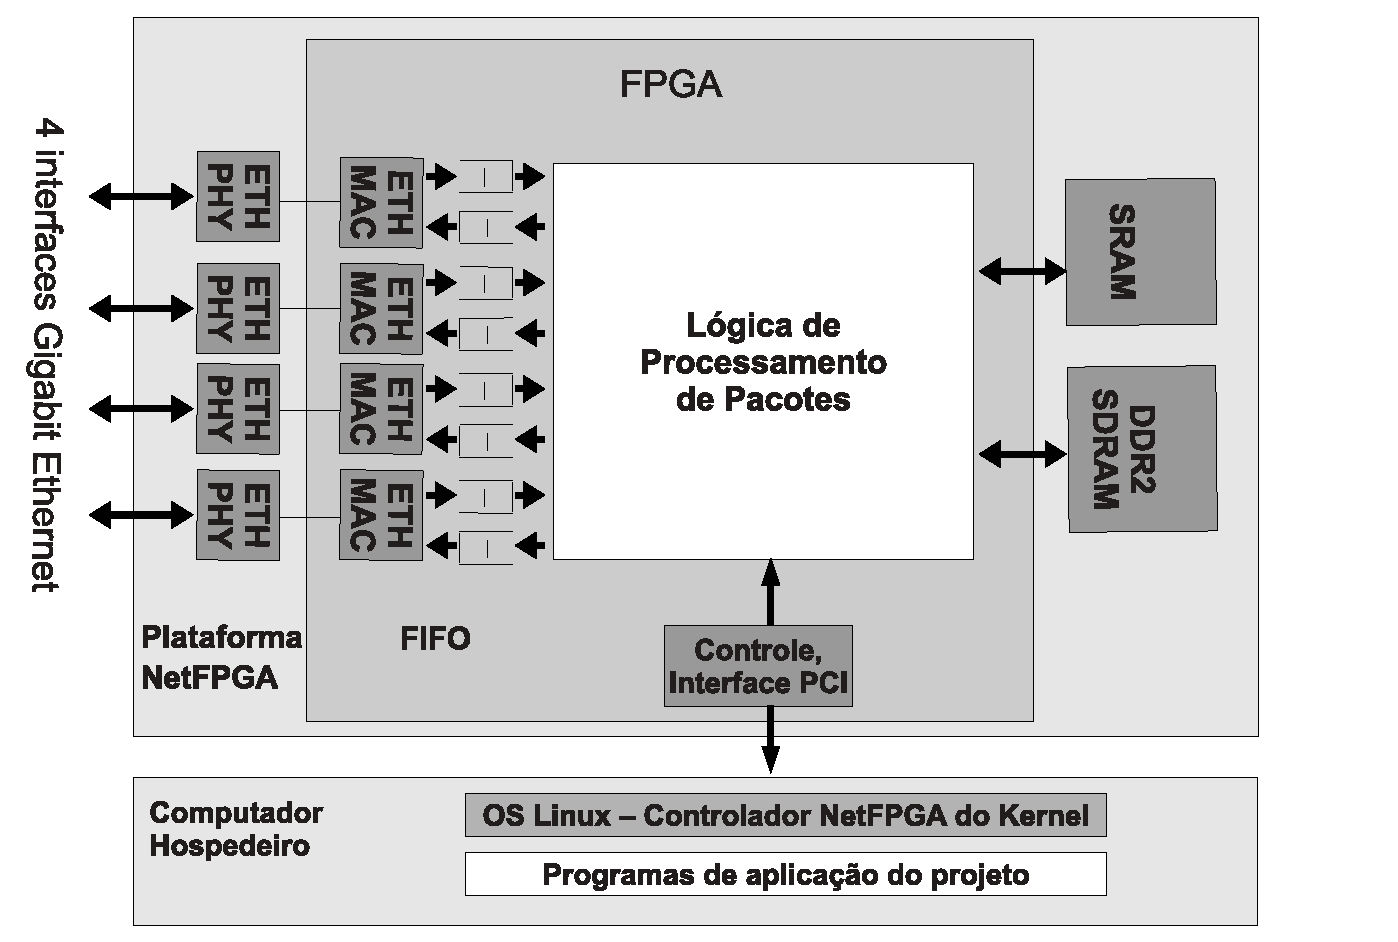
\includegraphics[scale=0.6,angle=0]{figures/placa/infraplaca.eps}
\caption{Componentes da NetFPGA.}
\label{fig:arch.hardware}
\end{figure}

A NetFPGA está disponível em outros modelos, todos com arquitetura
de \emph{hardware} similar composta de portas Ethernet, FPGA,
memória SRAM e memória DRAM.  As versões mais novas da NetFPGA
suportam Ethernet 10\,Gbps, FPGAs mais velozes e memórias de maior
capacidade.  Neste material iremos nos ater à NetFPGA 1G, que serve
como denominador comum e é de mais fácil acesso.  Os conceitos e
técnicas utilizados na NetFPGA 1G podem ser diretamente aplicados
aos outros modelos de NetFPGA.

\subsection{Software}
\label{sec:arch.soft}

A NetFPGA possui um pacote de \emph{software} construído para
facilitar o desenvolvimento de novos projetos.  Apesar da NetFPGA
permitir total flexibilidade no processamento de pacotes, a
arquitetura do \emph{hardware} é fixa e impõe limitações.  Como é de
se esperar, o \emph{software} da NetFPGA leva a arquitetura de
\emph{hardware} em consideração e apresenta uma série de interfaces
e abstrações que utilizamos para permitir modularização e
comunicação entre módulos.

\subsubsection{Projetos de referência}

A NetFPGA possui um conjunto de \emph{projetos de referência}, que a
fazem funcionar como uma placa de rede, um comutador Ethernet, ou um
roteador IP.  Nesta seção descrevemos os projetos de referência, que
servem de base para desenvolvimento de projetos mais complexos.

\subsubsection*{Placa de rede de referência}

A NetFPGA pode ser configurada como um conjunto de quatro interfaces
de rede utilizando o projeto \ssf{reference\_nic}.  Cada interface é
identificada pelo Linux como \ssf{nf2cX}, com \ssf{X} variando de
\ssf{0} a \ssf{3}.  Estas interfaces funcionam de forma análoga a
interfaces de rede como \ssf{eth0}, \ssf{wlan0}, e \ssf{lo}.

Pacotes de rede podem ser recebidos pelas interfaces \ssf{nf2cX}
pela porta Ethernet, quando outro computador envia um pacote através
da rede, ou pelo barramento PCI, quando o hospedeiro envia um pacote
que deve ser transmitido pela rede.  Para tratar o recebimento de
pacotes, o \ssf{reference\_nic} instancia oito módulos
\ssf{rx\_queue} para tratar recebimento de dados para cada interface
da porta Ethernet e barramento PCI ($4 \times 2 = 8$).  De forma
análoga, o \ssf{reference\_nic} instancia oito módulos
\ssf{tx\_queue} para tratar a transmissão de pacotes por cada
interface através da porta Ethernet e barramento PCI.  Os módulos
\ssf{rx\_queue} e \ssf{tx\_queue} fazem a interface entre o FPGA, o
controlador MAC e o controlador PCI.  A
\figstr~\ref{fig:arch.pipe.iface} mostra o \emph{pipeline} completo
de processamento do \ssf{reference\_nic}, com os módulos
\ssf{rx\_queue} e \ssf{tx\_queue} nas extremidades.

\begin{figure}
\centering
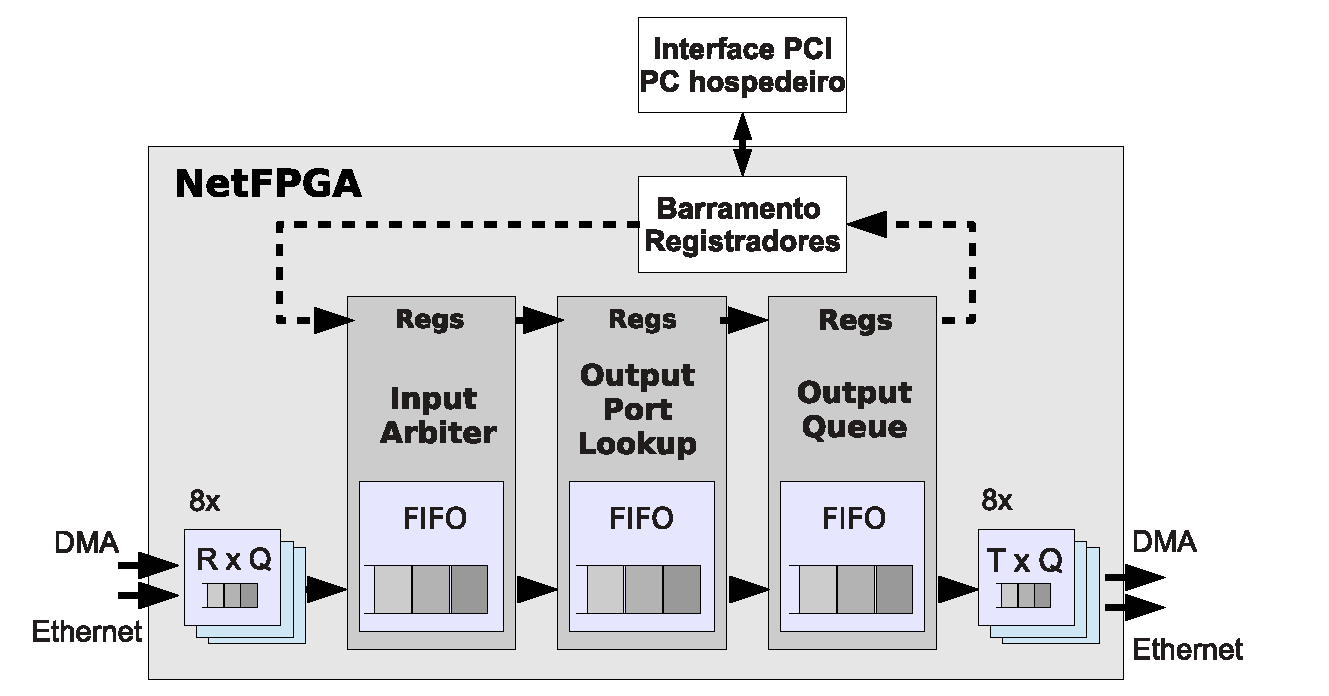
\includegraphics[scale=0.6,angle=0]{figures/modulos/datapathhor2.eps}
\caption{Pipeline de referência da NetFPGA configurada como interfaces de rede padrão.}
\label{fig:arch.pipe.iface}
\end{figure}

O processamento de pacotes na NetFPGA é realizado serialmente em um
\emph{pipeline} de múltiplos estágios.  Pacotes de rede são
retirados das filas de chegada (\ssf{rx\_queue}) pelo módulo
\ssf{input\_arbiter}.  O \ssf{input\_arbiter} decide qual fila de
chegada deve ser servida, retira o pacote da fila e o coloca no
\emph{pipeline} de processamento.  A política padrão de serviço é
iterar sequencialmente através de todas as filas de chegada.  Ao
colocar o pacote no \emph{pipeline} de processamento, o
\ssf{input\_arbiter} adiciona um meta-cabeçalho ao pacote indicando
em qual porta ele chegou e o envia para o próximo módulo no
\emph{pipeline} de processamento.

O próximo módulo no \emph{pipeline} é o \ssf{output\_port\_lookup},
que decide a porta de saída do pacote, adiciona essa informação no
meta-cabeçalho do pacote e o envia para o próximo módulo no
\emph{pipeline}.  A decisão da porta de saída do pacote em geral
depende dos endereços IP e MAC do destino, mas podem depender também
de outras propriedades do pacote.  Por exemplo, em nosso
\emph{firewall} o destino de pacotes TCP depende da porta de
destino.  O próximo módulo no \emph{pipeline} é o
\ssf{output\_queues}, que demultiplexa o pacote do \emph{pipeline}
de processamento nas filas de saída (\ssf{tx\_queue}).

A interface de comunicação entre os módulos do \emph{pipeline} de
processamento, por exemplo como mostrado na
\figstr~\ref{fig:arch.pipe.sinais}, é padronizada.  Existem sinais
\ssf{wr} e \ssf{rdy} para controlar quando o módulo anterior está
pronto para transmitir dados e quando o módulo posterior está pronto
para receber, respectivamente.  Transmissão de dados de pacotes só
acontece quando os dois sinais estão ligados.  A interface tem ainda
8 linhas \ssf{ctrl} que carregam sinais de controle e 64 linhas
\ssf{data} que carregam dados.  Quando \ssf{ctrl} é zero estamos
transmitindo dados do pacote. Quando \ssf{ctrl} é diferente de zero
estamos transmitindo meta-cabeçalhos do pacote.  Para cada
meta-cabeçalho existe um valor de \ssf{ctrl}
pré-definido.\footnotemark{}   Desta forma, a NetFPGA processa até
64~bits de dados de pacote por ciclo de relógio.  Dado o ciclo de
relógio de 8\,ns, o processamento de um pacote de 1500\,B leva da
ordem de 2\,$\mu$s.  A \figstr~\ref{fig:arch.pipe.sinais} ainda
mostra que módulos podem ser logicamente separados em duas partes:
uma fila para armazenamento temporário de dados e circuito para
processamento do pacote.

\footnotetext{Por exemplo, o meta-cabeçalho criado pelo
\sssf{input\_arbiter} com informações sobre a recepção de um pacote
tem \sssf{ctrl} igual a \sssf{IO\_QUEUE\_STAGE\_NUM} (\sssf{0xFF}).}

\begin{figure}
\centering
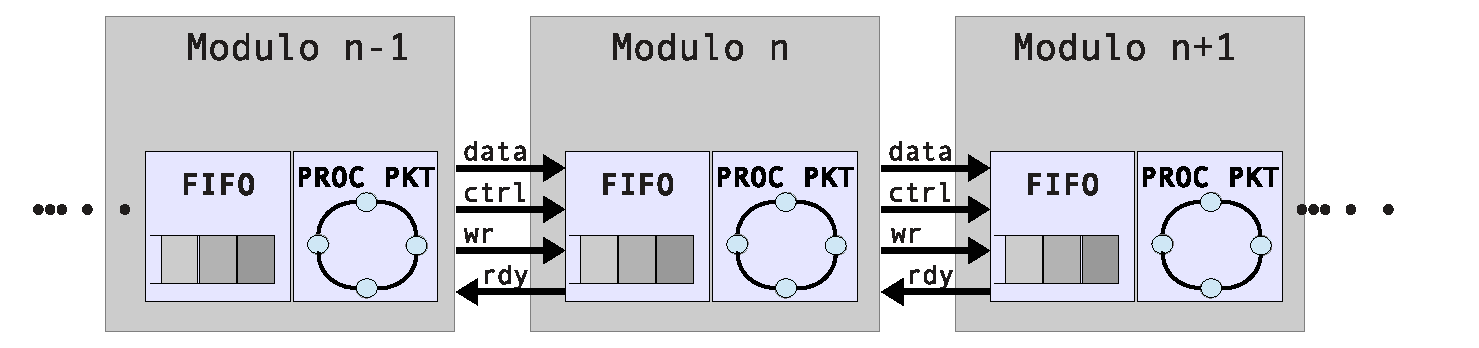
\includegraphics[scale=0.6,angle=0]{figures/modulos/fifo.eps}
\caption{Barramento de encaminhamento de pacotes.}
\label{fig:arch.pipe.sinais}
\end{figure}


\subsubsection*{Comutador de referência}

O comutador de referência (\ssf{reference\_switch}) reutiliza vários
dos módulos apresentados na descrição da placa de rede de
referência.  O único módulo com diferenças é o
\ssf{output\_port\_lookup}.  No comutador de referência, o módulo
\ssf{output\_port\_lookup} associa o endereço MAC da origem à porta
Ethernet de entrada toda vez que recebe um pacote.  Esta associação
é utilizada pelo \ssf{output\_port\_lookup} para decidir em qual
porta Ethernet enviar um pacote, verificando em qual porta o
endereço MAC do destino foi observado.

\subsubsection*{Roteador de referência}

Assim como o comutador de referência, o roteador de referência
(\ssf{reference\_router}), também reutiliza vários módulos
apresentados na descrição da placa de rede de referência.  O
roteador de referência estende o módulo \ssf{output\_port\_lookup}
para decidir a porta e saída de pacotes consultando a tabela de
roteamento.  A tabela de roteamento é implementada utilizando
registradores no FPGA como memória ternária.\footnote{O módulo que
implementa esta funcionalidade está disponível em
\url{netfpga/lib/verilog/core/reference_router/cam_router}.}

Além de rotear pacotes utilizando a tabela de roteamento, o roteador
de referência precisa calcular rotas usando protocolos de roteamento
como OSPF e BGP.  Como esses protocolos são muito complexos para
serem implementados em \emph{hardware}, eles são implementados em
programas que executam no espaço do usuário.  Em outras palavras, o
roteador de referência implementa o encaminhamento de pacotes (plano
de dados) em \emph{hardware} e implementa o cálculo de rotas (plano
de controle) em \emph{software}.\footnote{O programa que implementa
o plano de controle do roteador de referência é chamado de SCONE e é
armazenado em \url{netfpga/projects/scone/}.} Como rotas precisam
ser recalculadas apenas quando há mudanças na topologia da rede,
recalculá-las em \emph{software} não compromete a latência nem a
vazão do encaminhamento de pacotes.

Protocolos de roteamento calculam o próximo roteador que deve ser
utilizado para encaminhar um pacote até seu destino.  O próximo
roteador no caminho é identificado pelo seu endereço IP.  Para que o
roteador de referência possa efetivamente encaminhar o pacote para o
próximo roteador, ele precisa converter o endereço IP do próximo
roteador num endereço MAC.  Esta operação é realizada pelo protocolo
ARP.  O plano de controle do roteador de referência também executa o
protocolo ARP para informar ao módulo \ssf{output\_port\_lookup}
quais endereços MAC devem ser utilizados no encaminhamento de
pacotes.

\subsubsection{Estrutura de diretórios}

Para facilitar a navegação do pacote de \emph{software} da NetFPGA,
mostramos abaixo a estrutura de diretórios do pacote e uma breve
descrição do conteúdo de cada diretório.

\begin{verbnobox}[\footnotesize]
netfpga                {Diretório raiz}
   bin                 {Scripts para simulação, síntese e geração de registradores}
   bitfiles            {Diretório dos arquivos .bit dos projetos}
   lib                 {Bibliotecas de módulos e funções de simulação}
      C                {Bibliotecas C}
      java             {Biliotecas Java}
      Makefiles        {Arquivos makefile pré-definidos para simulação/síntese}
      Perl5            {Bibliotecas Perl}
      python           {Bibliotecas Python}
      release          {Arquivos XML de configuração global}
      scripts          {Scripts para configutação e testes da plataforma}
      verilog          {Módulos em Verilog para síntese}
         contributed   {Módulos Verilog de contribuidores}
         core          {Módulos Verilog oficiais}
      xml              {Arquivos XML de módulos}
   projects            {Diretório de projetos}
\end{verbnobox}

O diretório \ssf{bin} possui alguns programas de configuração do
ambiente de programação, sintetização de projetos bem como execução
de simulações e testes.  O diretório \ssf{bitfiles} contém imagens
de projetos depois de sintetizados, pontos para gravação na NetFPGA.
Como exemplo, podemos configurar a NetFPGA com a placa de rede de
referência executando:

\begin{verbnobox}
bin/nf_download bitfiles/reference_nic.bit
\end{verbnobox}

O diretório \ssf{lib} contém o código fonte do \emph{software}.  Por
exemplo, o fonte do programa \ssf{nf\_download} é armazenado em
\ssf{netfpga/lib/C/download}.  Dentro do diretório \ssf{lib}, o
subdiretório \ssf{lib/verilog/core} armazena os módulos do núcleo da
arquitetura da NetFPGA.  Os módulos do núcleo incluem módulos como
\ssf{rx\_queue}, \ssf{tx\_queue}, \ssf{input\_arbiter},
\ssf{output\_port\_lookup}, \ssf{output\_queues} e vários outros.

A pasta \ssf{projects} contém os projetos montados pela NetFPGA.
Cada projeto, inclusive os projetos de referência, seguem a seguinte
árvore de diretórios.

\begin{verbnobox}[\footnotesize]
   projects
      <project>        {Seu projeto}
         doc           {Documentação}
         include       {project.xml, XML de módulos criados}
         lib           {Arquivos de cabeçalho Python, Perl e C}
         src           {Módulos Verilog criados}
         sw            {Programas para teste do projeto}
         synth         {Diretório de arquivos de síntese}
         test          {Programas para testes do hardware e software em Python}
\end{verbnobox}

O diretório \ssf{doc} é utilizado para armazenar documentação do
projeto.  A pasta \ssf{include} é utilizada para armazenar os
arquivos XML de configuração; por exemplo, estes arquivos são lidos
pelo programa \ssf{nf\_register\_gen} para alocação e mapeamento dos
registradores.\footnote{O arquivo \sssf{include/project.xml} define
todos os módulos que serão instanciados no projeto, os demais
arquivos XML contém informações dos módulos implementados pelo
usuário.}  A pasta \ssf{lib} contém os cabeçalhos C, Perl e Python
necessários para utilizar os demais programas do \emph{software} da
NetFPGA com este projeto.\footnotemark{} A pasta \ssf{src} contém os
módulos em Verilog implementados pelo usuário.  Os módulos nesse
diretório podem estender e ter o mesmo nome dos módulos disponíveis
em \ssf{netfpga/lib/verilog/core}; neste caso, os módulos estendidos
tem prioridade sobre as versões originais.  As pastas \ssf{sw} e
\ssf{test} possuem programas e especificações de testes de regressão
do projeto.  Por último, a pasta \ssf{synth} contém arquivos de
síntese do projeto.  Iremos entrar em maiores detalhes das
informações relativas a um projeto e novos módulos Verilog na
seção~\ref{sec:impl}.

\footnotetext{Um exemplo de informação nos cabeçalhos C, Perl e
Python são os identificadores de registradores.}

\subsection{Interação hardware--software}

Para facilitar a interação entre os componentes de \emph{hardware} e
\emph{software,} o projeto da NetFPGA possui algumas interfaces.
Aqui descrevemos a interface de registradores e de memória que
servem para ler e escrever dos registradores e componentes de
memória, respectivamente.

\subsubsection{Interface de registradores}
\label{sec:arch.regs}

O \emph{software} da NetFPGA define três tipos de registradores:
contadores, registradores de \emph{software} e registradores de
\emph{hardware}.  Registradores armazenam valores arbitrários.
Contadores suportam as operações de incremento, decremento, e
zerar-ao-ler (\emph{reset-on-read}).  Contadores podem ser escritos
pela NetFPGA e lidos por um programa de usuário.  Registradores de
\emph{software} podem ser escritos por programas de usuário e lidos
pela NetFPGA e registradores de \emph{hardware} são escritos pela
NetFPGA e lidos por programas de usuário.

Registradores de um módulo são definidos dentro do arquivo XML de
configuração do modulo.  O arquivo XML define as propriedades (tipo,
nome e descrição) de cada registrador do módulo.  Há nove tipos de
registradores pré-definidos no \emph{software} da NetFPGA, mais um
tipo vetor de tamanho variável, como mostrado na
tabela~\ref{tab:arch.regs.types}.


\begin{table}[h]
\centering
\begin{tabular}{lr}
\textsc{Tipo} & \textsc{Bits} \\
\ssf{ethernet\_addr}      & 48 \\
\ssf{ip\_addr}            & 32 \\
\ssf{counter32}           & 32 \\
\ssf{software32}          & 32 \\
\ssf{generic\_counter32}  & 32 \\
\ssf{generic\_hardware32} & 32 \\
\ssf{generic\_sofware32}  & 32 \\
\ssf{dataword}            & 64 \\
\ssf{ctrlword}            & 8 \\
\ssf{vetor}                     & variável \\
\end{tabular}
\caption{Tipos de registradores e exemplos de definição.}
\label{tab:arch.regs.types}
\end{table}

\newpage{}

O \emph{software} da NetFPGA provê um programa que processa os
arquivos XML de todos os módulos de um projeto, identifica os
requisitos de memória para armazenamento dos registradores de cada
módulo e gera endereços para todos os registradores do projeto.
Este programa também gera arquivos de cabeçalho para as linguagens
Verilog, C, Perl e Python para permitir referências aos
registradores do projeto bem como em programas de usuário,
simulações e testes.

\subsubsection{Interface de memória}

A NetFPGA possui dois tipos de memória: SRAM e DRAM.  A memória SRAM
executa no mesmo ciclo de relógio do FPGA e leva três ciclos para
completar acessos, mas totaliza 4.5~MiB.  A DRAM funciona de forma
assíncrona ao FPGA e leva mais ciclos de relógio para completar
acessos, mas totaliza 64~MiB.  Apesar da maior latência no acesso à
DRAM, ela tem vazão suficiente para funcionar como área de
armazenamento temporário de pacotes, por exemplo nos módulos
\ssf{rx\_queue} e \ssf{tx\_queue}.

O controle do acesso à memória SRAM é realizado por um submódulo
chamado \ssf{sram\_arbiter}.  A tarefa principal do
\ssf{sram\_arbiter} é intermediar requisições de acesso à memória
recebida de vários módulos e da interface de registradores.  O
\ssf{sram\_arbiter} pode ser modificado para arbitrar o acesso à
memória de diferentes formas, dando prioridades distintas a módulos
de um projeto ou para otimizar o acesso à memória caso a aplicação
tenha padrões de acessos bem definidos.  Apesar da SRAM ter tempo de
acesso de três ciclos de relógio, o tempo de acesso total através do
\ssf{sram\_arbiter} depende do mecanismo de arbitragem utilizado.
Para permitir acesso concorrente à SRAM por diferentes módulos, o
\ssf{sram\_arbiter} armazena as requisições de acesso numa fila
interna.  Detalharemos o funcionamento do \ssf{sram\_arbiter} na
seção~\ref{sec:impl.mem}.



\newpage
\section{Implementação de um \emph{firewall} na NetFPGA}
\label{sec:impl}

Nesta seção apresentamos o \emph{firewall} que implementamos na
NetFPGA.  Apresentamos os detalhes de implementação e explicamos os
fundamentos para que o leitor possa implementar seu próprios
projetos.  Nosso \emph{firewall} tem várias simplificações para
torná-lo mais didático.  Em particular, o \emph{firewall} filtra
apenas pacotes TCP e o único tipo de regra que suporta é filtragem
por porta de destino.  Outra simplificação é que o \emph{firewall}
suporta filtragem de até quatro portas.  As razões destas
simplificações ficarão claras durante as discussões nesta seção.
Apesar das simplificações, esperamos que leitores sejam capazes de
estender o \emph{firewall} apresentado utilizando o conteúdo do
tutorial.

Esta seção é dividida em cinco partes complementares.  Na
\secstr~\ref{sec:impl.pkt} nós discutimos o processamento de pacotes
na NetFPGA, na \secstr~\ref{sec:impl.mod} discutimos como pacotes
podem ser modificados em trânsito, na \secstr~\ref{sec:impl.mem}
mostramos como um módulo pode utilizar a memória SRAM e na
\secstr~\ref{sec:impl.regs} mostramos como definir registradores e
acessá-los através de programas de espaço de usuário.  Por fim, na
\secstr~\ref{sec:impl.test} apresentamos o sistema de testes
disponível no \emph{software} da NetFPGA.

A maior parte do código apresentado neste material refere-se aos
arquivos Verilog (\ssf{.v}) usados para simulação e síntese do
\emph{hardware}.  A sintaxe para comentários em Verilog é idêntica à
de C.\footnotemark{}  O \emph{software} da NetFPGA possui também
\emph{scripts} Bash (\ssf{.sh}), Perl (\ssf{.pl}) e Python
(\ssf{.py}), que adotam o caractere (\ssf{\#}) para comentários de
linha.  Salvo quando indicado, iremos mostrar código retirado do
módulo principal do nosso \emph{firewall}, em
\ssf{netfpga/projects/firewall/src/firewall.v}.

\footnotetext{Algumas dicas para programação em Verilog são
apresentadas no apêndice A.}

\subsection{Processamento de pacotes}
\label{sec:impl.pkt}

Nesta seção iremos mostrar como pacotes são repassados entre módulos bem
como seu conteúdo pode ser acessado para uso em tomada de decisão ou
coleta de dados.

\subsubsection{Barramento de encaminhamento}

Nosso \emph{firewall} é construído como uma extensão do projeto de placa
de rede de referência. O processamento de pacotes é realizado por uma
sequência de módulos. O \emph{firewall} é instanciado no módulo
\ssf{user\_data\_path}, que define o \emph{pipeline} de processamento,
entre os módulos \ssf{output\_port\_lookup} e \ssf{output\_queues} (ver
figura~\ref{fig:arch.pipe.iface}).

Dados dos pacotes são transmitidos entre módulos através do barramento
de encaminhamento.  Como descrito na seção~\ref{sec:arch.soft} e
ilustrado na figura~\ref{fig:arch.pipe.sinais}, o barramento de
encaminhamento é composto de 64~bits de dados (\ssf{data}), 8~bits de
controle (\ssf{ctrl}), um bit para informar que o módulo anterior tem
dado disponível para enviar (\ssf{wr}) e um bit para informar que o
módulo está pronto para receber (\ssf{rdy}).  A definição das linhas de
comunicação do barramento de encaminhamento em nosso \emph{firewall} é
mostrada abaixo:

\begin{verilogcode}
module firewall
   #(
      parameter DATA_WIDTH = 64,
      parameter CTRL_WIDTH = DATA_WIDTH/8,
      ...
   )
   (
      input [DATA_WIDTH-1:0]              in_data,
      input [CTRL_WIDTH-1:0]              in_ctrl,
      input                               in_wr,
      output                              in_rdy,
      output reg [DATA_WIDTH-1:0]         out_data,
      output reg [CTRL_WIDTH-1:0]         out_ctrl,
      output reg                          out_wr,
      input                               out_rdy,
      ...
\end{verilogcode}

Todos os módulos do \emph{pipeline} de processamento da NetFPGA, como os
módulos \ssf{output\_port\_lookup} e \ssf{output\_queues}, possuem uma
fila que armazena dados de pacotes recebidos do módulo antecessor.  A
transferência entre módulos só é realizada quando ambos sinais \ssf{wr}
e \ssf{rdy} estão ligados.  Quando o bit \ssf{wr} não está ligado, o
módulo anterior não tem dados para transferir, por exemplo, por que a
placa não recebeu nenhum pacote.  Quando o bit \ssf{rdy} não está
ligado, a fila de recepção do módulo está cheia e ele não pode receber
mais dados, por exemplo, porque o processamento de um pacote está
demorando mais do que o esperado.  Note que quando um módulo não pode
receber dados, ele pode travar todo o \emph{pipeline} de processamento.
Em nosso \emph{firewall}, a fila que armazena os dados de pacotes
transmitidas pelo módulo anterior é uma instância de
\ssf{fallthrough\_small\_fifo} chamada \ssf{input\_fifo}:

\begin{verilogcode}
   fallthrough_small_fifo #(
      ...
   ) input_fifo (
      .din           ({in_ctrl, in_data}), // Data in
      .wr_en         (in_wr),              // Write enable
      .dout          ({in_fifo_ctrl, in_fifo_data}),
      .rd_en         (in_fifo_rd_en),      // Next word
      .nearly_full   (in_fifo_nearly_full),
      .empty         (in_fifo_empty),
      ...
\end{verilogcode}

A entrada da fila, \ssf{din}, é ligada diretamente às linhas de entrada
\ssf{in\_data} e \ssf{in\_ctrl}.  O controle do recebimento de dados no
barramento de processamento é realizado em duas partes.  Primeiro,
ligamos o sinal que informa se o módulo anterior tem dados para
escrever, \ssf{in\_wr}, diretamente no controle de escrita da fila,
\ssf{wr\_en} (linha 5).  Segundo, ligamos o sinal que informa se nosso
módulo pode receber dados, \ssf{in\_rdy}, diretamente no sinal que
informa se a fila está quase cheia (apenas uma posição livre):

\begin{verilogcode}
      assign in_rdy = !in_fifo_nearly_full;
\end{verilogcode}

Se o módulo anterior não tiver dados para enviar ou se a fila estiver
cheia, nada é escrito na fila.  Mais precisamente, se a fila estiver
cheia, nada será escrito na fila e o módulo anterior irá armazenar o
dado até a fila poder recebê-lo.

Como veremos na subseção seguinte, nosso \emph{firewall} retira dados da
fila lendo os dados em \ssf{in\_fifo\_data} e \ssf{in\_fifo\_ctrl},
ligados à saída da fila (\ssf{dout}), e ligando o sinal
\ssf{in\_fifo\_rd\_en} para avançar a fila para a próximo dado.

Os bits de controle, \ssf{in\_fifo\_ctrl}, especificam como os bits de
dados devem ser processados.  Os bits de controle possuem valor zero
enquanto o pacote está sendo transmitido.  Bits de controle diferentes
de zero denotam metadados que precedem ou sucedem os dados do pacote.  O
valor dos bits de controle define a semântica dos bits de dados,
\ssf{in\_fifo\_data}.  Por exemplo, quando os bits de controle valem
\ssf{IO\_QUEUES\_STAGE\_NUM} (\ssf{0xff}), os bits de dados contém
informações sobre o recebimento do pacote, por exemplo, em qual porta
Ethernet ele chegou.  Estes metadados podem ser utilizados no
processamento do pacote.

% \begin{figure}
% \centering
% 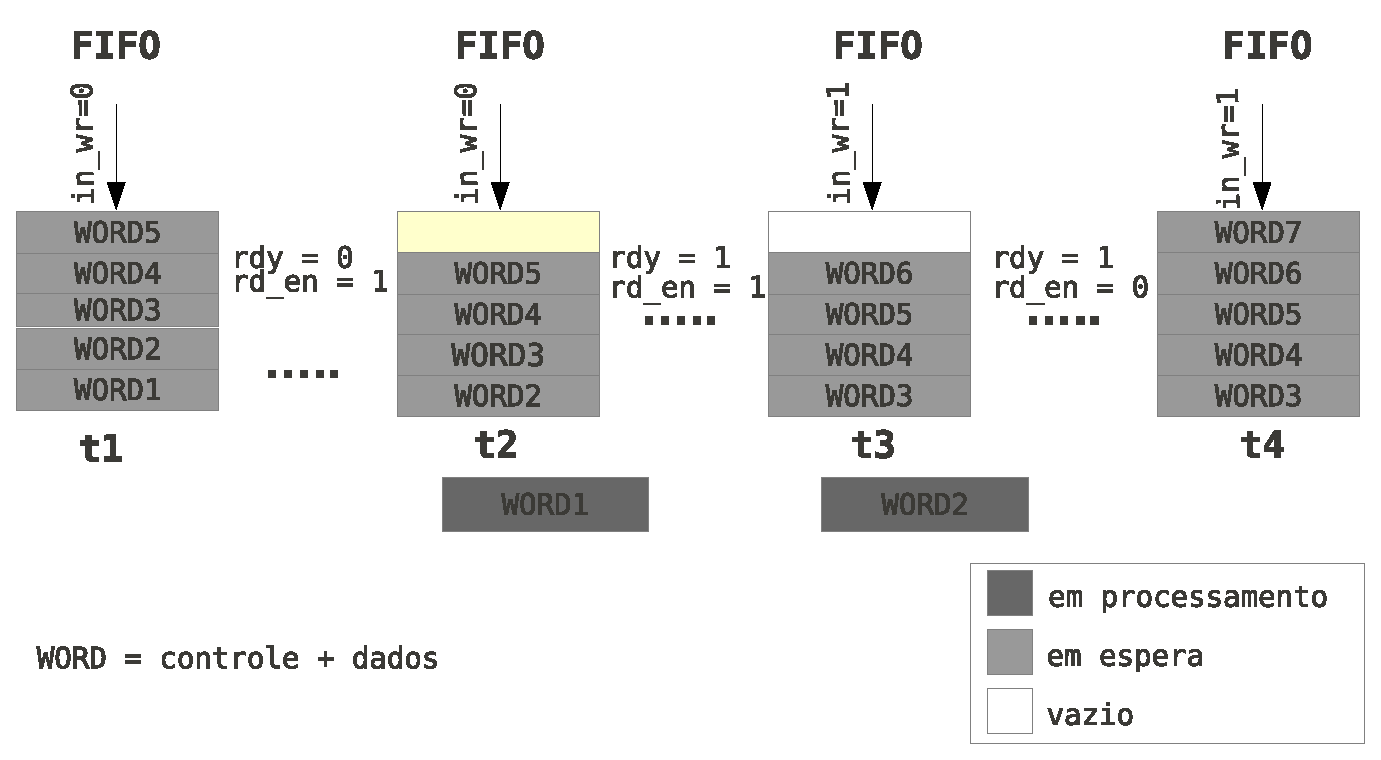
\includegraphics[scale=0.6,angle=0]{figures/modulos/fallthroughfifo.eps}
% \caption{Controle da fila de dados.}
% \label{fig:impl.fifo.msg}
% \end{figure}

\subsubsection{Máquina de estados}

Nosso \emph{firewall} implementa uma máquina de estados para verificar
se o pacote é IP e TCP.  Em caso positivo, a máquina de estados verifica
se a porta de destino deve ser filtrada e decide entre encaminhar ou
descartar o pacote.

Como todo o pacote é transmitido no barramento de encaminhamento com os
bits de controle zerados, nossa máquina de estado precisa manter
informação de qual palavra de 64~bits está sendo recebida.  Por exemplo,
como o cabeçalho IP e TCP somam pelo menos 40~bytes (56 bytes
contabilizando o cabeçalho Ethernet), o cabeçalho do pacote é recebido
ao longo de pelo menos cinco ciclos de relógio.  A
tabela~\ref{tab:impl.state.pktwords} mostra quais dados são transferidos
no barramento de encaminhamento a cada ciclo de relógio quando as linhas
de controle estão zeradas.

\begin{table}
\centering
\begin{tabular}{c|p{2.9cm}|p{2.9cm}|p{2.9cm}|p{2.9cm}|}
& \multicolumn{4}{c}{\ssf{in\_data}} \\
	Palavra & \multicolumn{1}{|c|}{\ssf{63:48}}     & \multicolumn{1}{|c|}{\ssf{47:32}}     & \multicolumn{1}{|c|}{\ssf{31:16}} & \multicolumn{1}{|c|}{\ssf{15:0}} \\ \hline
	1       & \multicolumn{3}{|l|}{Eth source addr} & Eth dest addr \\ \hline
	2       & \multicolumn{2}{|l|}{Eth dest addr}   & EtherType                             & IPver, HL, ToS \\ \hline
	3       & packet size                          & IP ID                                 & flags, frag                       & TTL, proto \\ \hline
	4       & checksum                             & \multicolumn{2}{|c|}{source IP}       & destination IP \\ \hline
	5       & destination IP                              & source port                          & destination port                         & seq. no. \\ \hline
	6       & seq. no.                             & \multicolumn{2}{|c|}{acknowledgement} & flags \\ \hline
	7       & adv. window                          & checksum                              & urgent ptr.                       & payload \\ \hline
	$\cdots$ & \multicolumn{4}{|l|}{payload} \\
\end{tabular}
\caption{Pacotes são encaminhados em palavras de 64 bits ao longo de
vários ciclos de relógio.  Na tabela um exemplo de pacote TCP.}
\label{tab:impl.state.pktwords}
\end{table}

\subsubsection*{Visão geral e atribuições padrão}

A figura~\ref{fig:impl.state.machine} mostra a máquina de estados do
nosso \emph{firewall}.  A ideia básica é receber o cabeçalho do pacote
para verificar se ele precisa ser descartado antes de transmiti-lo ao
próximo módulo.  Para receber e armazenar o cabeçalho do pacote
precisamos de uma fila de saída auxiliar, onde colocamos as palavras de
dados que já recebemos até decidir se devemos enviar o pacote para o
módulo seguinte ou descartá-lo.  A definição da fila de saída, mostrada
a seguir, é similar à definição da fila de entrada.

\begin{verilogcode}
   fallthrough_small_fifo #(
      ...
   ) output_fifo (
      .din           (out_fifo_din),   // Data in
      .wr_en         (out_fifo_wr),    // Write enable
      .rd_en         (out_fifo_rd_en), // Read the next word
      .dout          (out_fifo_dout),
      .full          (),
      .nearly_full   (out_fifo_nearly_full),
      .empty         (out_fifo_empty),
      .reset         (reset),
      .clk           (clk)
   );
\end{verilogcode}

A cada ciclo de relógio fazemos atribuições padrão que podem ser
sobrescritas dependendo do estado.  Em particular, deixamos a fila de
entrada travada, não escrevemos na fila de saída, e não repassamos dados
para o próximo módulo do \emph{pipeline}.  Também atribuímos os dados de
entrada da fila de saída aos dados retirados da fila de entrada.  Por
último, repassados ao próximo módulo no \emph{pipeline} os dados
retirados da fila de saída.

\begin{verilogcode}
    in_fifo_rd_en = 0;
    out_fifo_wr = 0;
    out_fifo_rd_en = 0;
    out_wr = 0;
    out_fifo_din = {in_fifo_ctrl, in_fifo_data};
    {out_ctrl, out_data} = out_fifo_dout;
\end{verilogcode}

\begin{figure}\centering
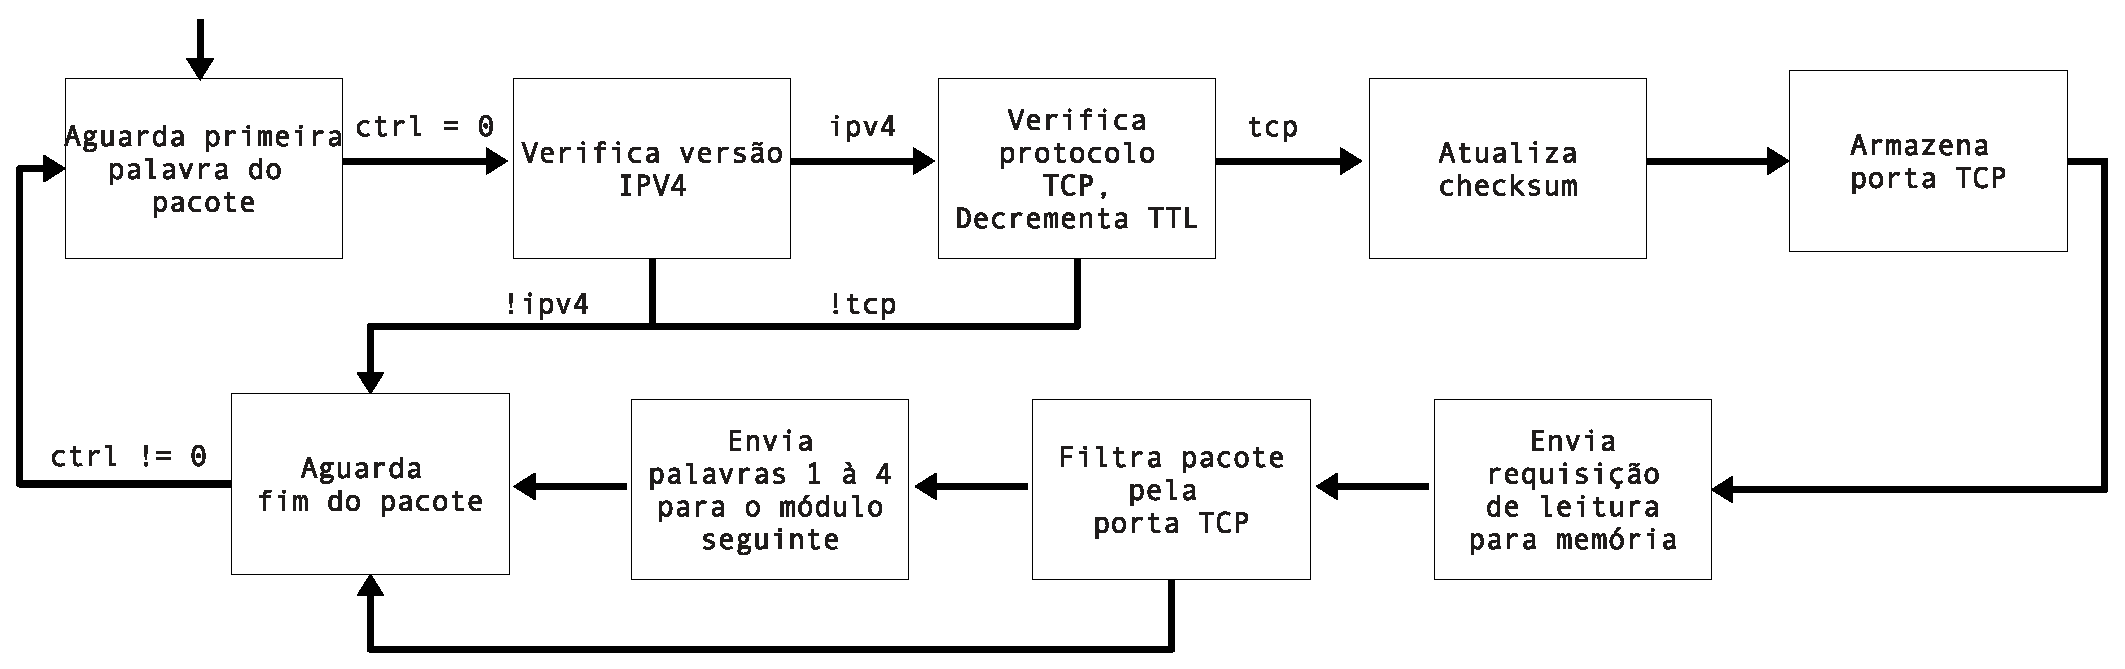
\includegraphics[scale=0.4]{figures/modulos/mestados.eps}
\caption{Máquina de estados do \emph{firewall}.}
\label{fig:impl.state.machine}
\end{figure}

Nossa máquina de estados atualiza todos os registradores a cada ciclo do
relógio.  Para cada registrador, temos um conjunto de linhas com o mesmo
nome e o sufixo \ssf{next}.  As linhas com sufixo \ssf{next} são
atribuídas aos respectivos registradores a cada ciclo do relógio.  Para
manter os valores nos registradores, inicializamos as linhas \ssf{next}
com o valor atual dos registradores e modificamos o valor das linhas
\ssf{next} em estados específicos quando necessário.

\subsubsection*{Primeiro estado: esperando o início de pacotes}

O primeiro estado da nossa máquina de estados, \ssf{WAIT\_PACKET},
simplesmente espera o início do recebimento de um pacote, isto é,
espera as linhas de controle serem zeradas.  A implementação do
primeiro estado, mostrada abaixo, primeiro verifica se existe pacote
a processar e se o próximo módulo está pronto para receber pacotes
verificando \ssf{in\_fifo\_empty} e \ssf{out\_rdy}, respectivamente.
Se não há dado a processar ou se o próximo módulo não está pronto
para receber, continuamos neste estado sem avançar as filas de
entrada e saída (linha 12).  Se há dado a processar e o próximo
módulo está pronto para recebê-lo, nossa máquina de estados avança a
fila ligando o sinal \ssf{in\_fifo\_rd\_en} e grava os dados na fila
de saída ligando \ssf{out\_fifo\_wr}.  Se os bits de controle
\ssf{in\_fifo\_ctrl} não estiverem zerados, significa que ainda
estamos recebendo metadados e o início do pacote ainda não chegou.
Quando os bits de controle estiverem zerados significa que acabamos
de receber a primeira palavra de dados do pacote (que contém o
endereço MAC da origem, tabela~\ref{tab:impl.state.pktwords}) e
passamos para o segundo estado.

\begin{verilogcode}
  WAIT_PACKET: begin
     if (!in_fifo_empty && out_rdy) begin
        in_fifo_rd_en = 1;
        out_fifo_wr = 1;
        if(in_fifo_ctrl == 'h0) begin
           state_next = WORD2_CHECK_IPV4;
        end else begin
           state_next = WAIT_PACKET;
        end
     end
     else
        state_next = WAIT_PACKET;
  end
\end{verilogcode}


\subsubsection*{Segundo estado: verificação do protocolo de rede}

O segundo estado nosso \emph{firewall} processa a segunda palavra do
pacote e verifica se o pacote é um pacote IPv4.  Para isso
verificamos se o tipo do cabeçalho Ethernet (EtherType) é
\ssf{0x0800}, que indica um pacote IP, e se a versão do protocolo IP
é \ssf{4}.\footnotemark{} Em caso positivo, prosseguimos para o
próximo estado para verificar se o pacote é um pacote TCP.  Caso o
pacote não seja um pacote IPv4 ele deverá ser encaminhado pela rede
sem ser filtrado.  Para encaminharmos o pacote pulamos para o oitavo
estado, \ssf{EMPTY\_OUT\_FIFO}, descrito abaixo.

\footnotetext{Note que nosso \emph{firewall} não suporta VLANs
(802.1Q).  Para tal seria necessário considerar o caso onde o
EtherType é \ssf{0x8100}.}

\begin{verilogcode}
  WORD2_CHECK_IPV4: begin
     if (!in_fifo_empty && out_rdy) begin
        if(in_fifo_data[31:16] != 16'h0800 ||
              in_fifo_data[15:12] != 4'h4) begin
           state_next = EMPTY_OUT_FIFO;
        end
        else begin
           in_fifo_rd_en = 1;
           out_fifo_wr = 1;
           state_next = WORD3_CHECK_TCP_TTL;
        end
     end
     else
        state_next = WORD2_CHECK_IPV4;
  end
\end{verilogcode}

\subsubsection*{Terceiro estado: verificação do protocolo de transporte}

No terceiro estado inspecionamos o cabeçalho IP para ver se o valor
do campo protocolo é \ssf{0x06}, que indica TCP.  Em caso negativo o
pacote é aceito: pulamos para o estado \ssf{EMPTY\_OUT\_FIFO} para
enviarmos as duas primeiras palavras mais metadados que foram
armazenadas na fila de saída (linha 9).  Note que, em caso negativo,
a fila de entrada fica bloqueada com a terceira palavra, que será
transmitida após esvaziarmos a fila de saída no estado
\ssf{EMPTY\_OUT\_FIFO}.  Em caso positivo, encaminhamos a terceira
palavra para a fila de saída e passamos para o próximo estado.

\begin{verilogcode}
  WORD3_CHECK_TCP_TTL: begin
     if (!in_fifo_empty && out_rdy) begin
        if(in_fifo_data[7:0] == 8'h06) begin
           in_fifo_rd_en = 1;
           out_fifo_wr = 1;
           state_next = WORD4_ADDR_CHKSUM;
        end
        else
           state_next = EMPTY_OUT_FIFO;
     end
     else
        state_next = WORD3_CHECK_TCP_TTL;
  end
\end{verilogcode}

\subsubsection*{Quarto estado: armazenamento dos endereços IP}

O quarto estado do \emph{firewall} armazena os dados da quarta
palavra do pacote temporariamente até verificarmos o número da porta
de destino no protocolo TCP no próximo estado.

\begin{verilogcode}
  WORD4_ADDR_CHKSUM: begin
     if (!in_fifo_empty && out_rdy) begin
        in_fifo_rd_en = 1;
        out_fifo_wr = 1;
        state_next = WORD5_TCP_PORT;
     end
     else
        state_next = WORD4_ADDR_CHKSUM;
  end
\end{verilogcode}

\subsubsection*{Quinto, sexto e sétimo estágios: verificando porta de
destino}

No quinto estado a fila de entrada contém a quinta palavra do
pacote, que possui o número da porta de destino do protocolo TCP.
Nós mantemos as filas de entrada e saída travadas, armazenamos a
porta de destino no registrador \ssf{dst\_port} e avançamos para o
próximo estágio.

\begin{verilogcode}
  WORD5_TCP_PORT: begin
     if (!in_fifo_empty && out_rdy) begin
        // in_fifo_rd_en and out_fifo_wr are zero by default
        dst_port_next = in_fifo_data[31:16];
        state_next = CHECK_RULES;
     end
     else
        state_next = WORD5_TCP_PORT;
  end
\end{verilogcode}

No sexto estágio mantemos as filas de entrada e saída travadas e
enviamos uma requisição de leitura da memória.  O endereço lido é
\ssf{SRAM\_PORTS\_ADDR}, que é definido igual a zero (primeira linha
da memória) e contém as portas de destino que estão bloqueadas.  Nós
lemos as portas bloqueadas da memória para ilustrar o acesso à
memória SRAM e porque as portas bloqueadas podem ser alteradas
assincronamente pelo usuário.  Na seção~\ref{sec:impl.mem} iremos
detalhar o acesso à memória.

\begin{verilogcode}
  CHECK_RULES: begin
     sram_rd_req_next = 1;
     sram_rd_addr_next = SRAM_PORTS_ADDR;
     state_next = CHECK_PORTS;
  end
\end{verilogcode}

Por último, o sétimo estágio espera a memória SRAM retornar os dados
verificando o valor de \ssf{rd\_vld}.  Esta espera é necessária pois
a SRAM demora alguns ciclos de relógio para retornar o dado
requisitado.  Uma versão otimizada do nosso \emph{firewall} poderia
realizar a requisição de memória antes para evitar esta espera.  Se
a porta de destino for uma das portas bloqueadas, ligamos o
registrador \ssf{drop}.  Independente da porta de destino passamos
para o próximo estágio, onde a fila de saída será esvaziada e os
dados transmitidos para o próximo módulo dependendo do valor do
registrador \ssf{drop}.

\begin{verilogcode}
      CHECK_PORTS: begin
         if (rd_0_vld) begin
            if(sram_rd_data[15:0] == dst_port ||
                   sram_rd_data[31:16] == dst_port ||
                   sram_rd_data[47:32] == dst_port ||
                   sram_rd_data[63:48] == dst_port)
               drop_next = 1;
            else
               drop_next = 0;
            state_next = EMPTY_OUT_FIFO;
         end
         else
            state_next = CHECK_PORTS;
      end
\end{verilogcode}

\subsubsection*{Oitavo estágio: processando palavras armazenadas
temporariamente}

O oitavo estágio é responsável por processar os metadados e dados do
pacote armazenados temporariamente na fila de saída para o módulo
seguinte do \emph{pipeline}.  A cada ciclo de relógio processamos
uma palavra da fila de espera (linha 6).  Se o registrador
\ssf{drop} estiver desligado, enviamos uma palavra da fila de espera
para o próximo módulo (linha 7).  Se o registrador \ssf{drop}
estiver ligado, retiramos os dados da fila sem repassá-los ao módulo
seguinte, efetivamente descartando o pacote.  Quando a fila de
espera estiver vazia pulamos para o último estado onde enviamos o
restante do pacote (a partir da quinta palavra) para o próximo
módulo diretamente da fila de entrada.

\begin{verilogcode}
      EMPTY_OUT_FIFO: begin
         if(!out_rdy)
            state_next = EMPTY_OUT_FIFO;
         else if(!out_fifo_empty) begin
            state_next = EMPTY_OUT_FIFO;
            out_fifo_rd_en = 1;
            out_wr = ~drop;
         end
         else
            state_next = PAYLOAD;
      end
\end{verilogcode}

\subsubsection*{Nono estágio: processando o conteúdo do pacote}

O nono e último estágio processa o resto do pacote a partir da fila
de entrada.  Os dados retirados da fila de entrada são repassados
para o próximo módulo dependendo do valor de \ssf{drop}.  Voltamos
para o primeiro estado quando detectamos o início do próximo pacote.
Detectamos o início do próximo pacote quando os bits de controle têm
o valor \ssf{IO\_QUEUE\_STAGE\_NUM}, do metadado adicionado pelas
filas de entrada quando o pacote é recebido na NetFPGA.  Note que
assim que detectamos o início do próximo pacote travamos a fila de
entrada para que a primeira palavra do pacote seja processada pelo
primeiro estado do \emph{firewall}.

\begin{verilogcode}
      PAYLOAD: begin
         if (!in_fifo_empty && out_rdy) begin
            {out_ctrl, out_data} = {in_fifo_ctrl, in_fifo_data};
            if(in_fifo_ctrl != `IO_QUEUE_STAGE_NUM)
                in_fifo_rd_en = 1;
                out_wr = ~drop;
                state_next = PAYLOAD;
            else begin
               in_fifo_rd_en = 0;
               out_wr = 0;
               drop_next = 0;            // reset drop register
               state_next = WAIT_PACKET;
            end
         end
         else
            state_next = PAYLOAD;
      end
\end{verilogcode}




\subsection{Modificação de pacotes em trânsito}
\label{sec:impl.mod}

Uma das funcionalidades da NetFPGA é a capacidade de modificar
pacotes em trânsito.  Iremos ilustrar essa funcionalidade
decrementando o tempo de vida (\emph{time to live}, TTL) do pacote.
Iremos também recalcular o \emph{checksum} do pacote.  Para tanto
vamos estender o código apresentado na subseção anterior.

O tempo de vida do pacote é transmitido na terceira palavra
(figura~\ref{tab:impl.state.pktwords}).  Nosso \emph{firewall}
processa a terceira palavra do pacote no quarto estado
(\ssf{WORD4\_ADDR\_TTL}).  Para decrementar o tempo de vida, iremos
modificar o dado do pacote antes de inseri-lo na fila de saída, como
segue:

\begin{verilogcode}
      WORD3_CHECK_TCP_TTL: begin
         if (!in_fifo_empty && out_rdy) begin
            if(in_fifo_data[7:0] == 8'h06) begin
               in_fifo_rd_en = 1;
               out_fifo_wr = 1;
               out_fifo_din = {in_fifo_ctrl, in_fifo_data[63:16],
                               in_fifo_data[15:8] - 8'h1,
                               in_fifo_data[7:0]};
               state_next = WORD4_ADDR_CHKSUM;
            end
            else
               state_next = EMPTY_OUT_FIFO;
         end
         else
            state_next = WORD3_CHECK_TCP_TTL;
      end
\end{verilogcode}

De forma similar, precisamos atualizar o \emph{checksum} do pacote
devido ao decremento do tempo de vida.  Como o \emph{checksum} do
protocolo IP é simplesmente uma soma, podemos atualizá-lo
simplesmente somando o que foi subtraído devido ao decremento do
tempo de vida.\footnotemark{} No código abaixo, \ssf{chksum} possui
17~bits para conseguirmos somar o \emph{carry out} em \ssf{\tt
chksum\_cout}, que possui 16~bits.

\footnotetext{O cálculo do \emph{checksum} do protocolo IP é
detalhado no RFC1071.  Ele depende do valor da soma das palavras de
2~bytes dos campos do cabeçalho usando complemento de um.  Como o
tempo de vida tem apenas 1~byte e está alinhado com o byte mais
significativo da palavra de 2~bytes que o contém, nós incrementamos
o byte mais significativo do \emph{checksum}, somando \sssf{0x0100},
para compensar.}

\begin{verilogcode}
      assign chksum = {0, in_fifo_data[63:48]} + 16'h0100;
      assign chksum_cout = chksum[15:0] + {15'h0, chksum[16]};
        ...
      WORD4_ADDR_CHKSUM: begin
        if (!in_fifo_empty && out_rdy) begin
            in_fifo_rd_en = 1;
            out_fifo_wr = 1;
            in_out_fifo_dout = {in_fifo_ctrl, chksum_cout,
                        in_fifo_data[47:0]};
            state_next = WORD5_TCP_PORT;
        end
        else
            state_next = WORD4_ADDR_CHKSUM;
      end
\end{verilogcode}


\subsection{Acesso à memória SRAM}
\label{sec:impl.mem}

Nosso módulo utiliza a memória SRAM para armazenar as portas
bloqueadas e decidir quais pacotes filtrar.  No sexto estado do
processamento de um pacote emitimos uma requisição de leitura para o
endereço \ssf{SRAM\_PORTS\_ADDR}, que contem as portas TCP
bloqueadas.  No sétimo estado esperamos a leitura completar e então
utilizamos o dado lido para verificar se o pacote precisa ser
descartado ou não.

Nosso \emph{firewall} emite operações de leitura da memória para o
módulo \ssf{sram\_arbiter}, que intermedia o acesso à memória SRAM.
As linhas de comunicação do nosso \emph{firewall} com o
\ssf{sram\_arbiter} ilustram a interface de acesso à memória.

\begin{verilogcode}
      output reg                       sram_rd_req,
      output reg [SRAM_ADDR_WIDTH-1:0] sram_rd_addr,
      input [DATA_WIDTH-1:0]           sram_rd_data,
      input                            sram_rd_ack,
      input                            sram_rd_vld,
      output reg                       sram_wr_req,
      output reg [SRAM_ADDR_WIDTH-1:0] sram_wr_addr,
      output reg [DATA_WIDTH-1:0]      sram_wr_data,
      input                            sram_wr_ack,
\end{verilogcode}

O \ssf{sram\_arbiter} pode receber uma requisição de leitura ou
escrita por ciclo de relógio.  Requisições de leitura são indicadas
ligando \ssf{sram\_rd\_req} e informando o endereço a ser lido em
\ssf{sram\_rd\_addr}.  No próximo ciclo de relógio o
\ssf{sram\_arbiter} indica se a requisição foi recebida com sucesso
ligando o sinal \ssf{sram\_rd\_ack}.  Como leituras demoram alguns
ciclos para serem atendidas, o módulo que pediu a leitura deve
esperar os dados serem retornados e disponibilizados pelo
\ssf{sram\_arbiter}.  O \ssf{sram\_arbiter} informa que os dados
estão disponíveis em \ssf{sram\_rd\_data} ligando
\ssf{sram\_rd\_vld}.

Requisições de escrita são indicadas ligando \ssf{sram\_wr\_req},
informando o endereço a ser escrito em \ssf{sram\_wr\_addr} e
informando o dado a ser escrito em \ssf{sram\_wr\_data}.  O
\ssf{sram\_arbiter} indica se a requisição foi recebida com sucesso
ligando o sinal \ssf{sram\_wr\_ack}.  Como o dado a ser escrito é
armazenado pelo \ssf{sram\_arbiter}, o módulo que fez a requisição
de escrita não precisa esperar mais nenhuma confirmação do
\ssf{sram\_arbiter}.  Se ambos os sinais \ssf{sram\_rd\_req} e
\ssf{sram\_wr\_req} estiverem ligados, nosso \ssf{sram\_arbiter}
prioriza a requisição de escrita.  A SRAM usada na NetFPGA garante
que leituras realizadas após escritas lerão o dado atualizado.

A interface que exportamos em nosso \ssf{sram\_arbiter} é
simplificada.  Como descrito na seção~\ref{sec:arch.hw}, a NetFPGA
possui dois bancos de memórias SRAM, cada um com $2^{19}$ linhas de
36~bits.  Nosso \ssf{sram\_arbiter} combina os dois bancos para
apresentar uma abstração de memória de $2^{19}$ linhas de 64~bits.
Usamos 8~bits de cada linha como bits de paridade, calculados e
verificados automaticamente pelo \ssf{sram\_arbiter}.

\begin{verilogcode}
   // sram_arbiter.v
   generate
      genvar m;
      for(m = 0; m < 8; m = m+1) begin: calc_par_bits
      assign parbit[m] = wr_data[m*8] ^ wr_data[m*8+1] ^
            wr_data[m*8+2] ^ wr_data[m*8+3] ^ wr_data[m*8+4] ^
            wr_data[m*8+5] ^ wr_data[m*8+6] ^ wr_data[m*8+7];
      end // wr_data is 64 bits wide
   endgenerate 
   generate
      genvar l;
      for(l = 0; l < 8; l = l+1) begin: expand_wr_data
         assign wr_data_exp[(l+1)*9-1 : l*9] =
            {wr_data[(l+1)*8-1:l*8], parbit[l]};
         end // wr_data_exp is 72 bits wide (36*2)
   endgenerate
\end{verilogcode}

Para acessar as duas memórias simultaneamente duplicamos os sinais
de requisição de escrita ou leitura e os endereços para os dois
bancos de memória.  Para requisições de escrita escrevemos metade
dos dados em cada banco e para requisições de leitura concatenamos
os dados dos dois bancos.  Abaixo mostramos o código para realizar
estas operações.  Este código fica dentro do módulo \ssf{nf2\_core}.
O módulo \ssf{nf2\_core} é o módulo raiz do \emph{software} da
NetFPGA e comunica diretamente com os pinos do FPGA.  O
\ssf{nf2\_core} conecta os pinos do FPGA conectados às memórias SRAM
ao \ssf{sram\_arbiter} da seguinte forma.

\begin{verilogcode}
// nf2_core.v
// hardware pins       sram_arbiter
assign sram1_wr_data = wr_data_exp[`SRAM_DATA_WIDTH-1:0];
assign sram2_wr_data = wr_data_exp[2*`SRAM_DATA_WIDTH-1:`SRAM_DATA_WIDTH];
assign sram1_we      = sram_we; // 0 for write, 1 for read
assign sram2_we      = sram_we;
assign sram1_addr    = sram_addr;
assign sram2_addr    = sram_addr;
// sram_arbiter        hardware pins
assign sram_rd_data  = {sram2_rd_data, sram1_rd_data};
\end{verilogcode}

O \ssf{sram\_arbiter} pode ser modificado para permitir acesso mais
eficiente à memória caso a aplicação tenha um padrão específico de
acessos.  Por exemplo, é possível modificar as atribuições acima
para permitir ler endereços distintos em cada banco de SRAM.  A SRAM
também provê um mecanismo para permitir escritas parciais,
escolhendo quais bytes devem ser escritos em uma requisição de
escrita.\footnotemark{}

\footnotetext{Não mostramos esta funcionalidade no texto.  Nossa
implementação não suporta escritas parciais.  Escritas parciais
poderiam ser controladas configurando o valor das linhas
\sssf{sram\_bw} no \sssf{sram\_arbiter}.}

Para exemplificar o controle de acesso à SRAM num nível mais baixo,
iremos explicar o tratamento de uma requisição de leitura
(requisições de escrita são mais simples).  Quando o
\ssf{sram\_arbiter} recebe uma requisição de leitura, ele desabilita
escrita ligando o sinal \ssf{sram\_we} (este sinal possui lógica
negativa), repassa o endereço a ser lido ao \emph{hardware} e
confirma a requisição de leitura.

\begin{verilogcode}
   // sram_arbiter.v
   else if(sram_rd_req) begin
      hw_we <= 1'b1;                // read
      hw_addr <= sram_rd_addr;
      sram_rd_ack <= sram_rd_req;   // acknowledge read request
      sram_wr_ack <= 0;             // do not acknowledge write
      rd_vld_early3 <= sram_rd_req; // data back in three cycles
      ...
   end
\end{verilogcode}

Como o dado demora dois ciclos para ser retornado da SRAM após a
requisição, o \ssf{sram\_arbiter} possui um \emph{pipeline} interno
para esperar os dados serem retornados pela SRAM.  Após dois ciclos
o \ssf{sram\_arbiter} armazena o dado lido no registrador
\ssf{sram\_rd\_data} e encaminha este registrador para o
\emph{firewall} no terceiro ciclo de relógio após a requisição.

\begin{verilogcode}
   // sram_arbiter.v
   rd_vld_early2 <= rd_vld_early3; // waited 1
   rd_vld_early1 <= rd_vld_early2; // waited 2
   if(rd_vld_early1) begin // memory sending data this cycle, storing
      if(parity_check)
         sram_rd_data <= rd_data_exp_parsed; // no parity bits
      else
         sram_rd_data <= 64'hdeadfeeddeadfeed;
   end
   sram_rd_vld <= rd_vld_early1;   // data is here, set valid bit
\end{verilogcode}


\subsection{Registradores e interface PCI}
\label{sec:impl.regs}

Nosso projeto define quatro registradores de \emph{software}, um
para cada porta de destino que deve ser bloqueada.  Estes
registradores de \emph{software} podem ser configurados
dinamicamente a partir do espaço de usuário.  Nós definimos os
registradores no arquivo XML de configuração do nosso projeto como
abaixo.

\begin{minted}{xml}
<!-- netfpga/projects/firewall/include/project.xml -->
<nf:name>firewall</nf:name>
   <nf:prefix>firewall</nf:prefix>
   <nf:location>udp</nf:location>
   <nf:description>Registers for minifirewall</nf:description>
   <nf:blocksize>128</nf:blocksize>
   <nf:registers>
      <nf:register>
         <nf:name>dport1</nf:name>
         <nf:description>Blocked port 1</nf:description>
         <nf:type>generic_software32</nf:type>
      </nf:register>
      ...
   </nf:registers>
\end{minted}

O programa \ssf{nf\_register\_gen} processa os arquivos XML de
configuração de todos os módulos de um projeto, gera um
identificador para cada módulo, calcula requisitos de armazenamento
para os registradores de cada módulo e gera endereços virtuais para
cada registrador.\footnotemark{}  O endereço virtual de um
registrador é composto do identificador do módulo onde foi declarado
e de seu deslocamento dentro do bloco de memória reservado aos
registradores do módulo.  Como nosso \emph{firewall} possui quatro
registradores de 32 bits para armazenar as portas TCP que estão
bloqueadas, definimos um bloco de registradores de 128 bits
(\ssf{blocksize} na configuração acima).  O tamanho do bloco de
registradores define a quantidade de bits necessárias para a parte
de deslocamento do endereço dos registradores.

\footnotetext{O arquivo XML com a configuração global do
\emph{firewall} está em
\url{netfpfa/projects/firewall/include/project.xml}.  Arquivos com a
configuração dos módulos estão no mesmo diretório.}

O \ssf{nf\_register\_gen} gera cabeçalhos Verilog, C, Python e Perl
contendo constantes que permitem endereçar os registradores em cada
uma destas linguagens.  Os arquivos de cabeçalho são necessários
para compilação de programas de usuário e sintetização do projeto em
\emph{hardware}.  O \ssf{nf\_register\_gen} pode ser executado com o
comando seguinte (os cabeçalhos são criados dentro da pasta
\ssf{netfpga/projects/firewall/lib/}):

\begin{minted}{bash}
netfpga/bin/nf_register_gen.pl --project firewall
\end{minted}

% \begin{table}[h]
% \centering
% \begin{tabular}{|l|l|l|}
% \hline
% \textbf{Macro}       & \textbf{Endereço Verilog} & \textbf{Endereço C} \\ \hline
% FIREWALL\_DPORT1 & 5'h0                      & 0x2000000           \\ \hline
% FIREWALL\_DPORT2 & 5'h1                      & 0x2000004           \\ \hline
% FIREWALL\_DPORT3 & 5'h2                      & 0x2000008           \\ \hline
% FIREWALL\_DPORT4 & 5'h3                      & 0x200000c           \\ \hline
% \end{tabular}
% \label{tab:impl.firewall.regs}
% \caption{Endereços virtuais em arquivos de cabeçalho C e Verilog dos registradores do firewall.}
% \end{table}

Os endereços virtuais de registradores em programas do usuário
possuem 28~bits e independem do tipo do registrador (contador,
\emph{software}, ou \emph{hardware}).  Como a NetFPGA interage com
sistemas operacionais de 32~bits, registradores maiores que 32 bits
são particionados em múltiplas palavras de 32~bits segundo o esquema
mostrado nas colunas ``64~bits'' e ``128~bits'' na
tabela~\ref{table:impl.regs.width}.

\begin{table}[h]
\centering
\begin{tabular}{llllll}
\multicolumn{2}{c}{\textbf{32 bits}} & \multicolumn{2}{c}{\textbf{64 bits}} & \multicolumn{2}{c}{\textbf{128 bits}} \\ \hline
\textbf{Macro}     & \textbf{Endereço} & \textbf{Macro}         & \textbf{Endereço} & \textbf{Macro}            & \textbf{Endereço} \\ \hline
\ssf{EX\_REG} & 0x2000004         & \ssf{EX\_REG\_LO} & 0x2000004         & \ssf{EX\_REG\_1\_LO} & 0x2000004   \\
                   &                   & \ssf{EX\_REG\_HI} & 0x2000008         & \ssf{EX\_REG\_1\_HI} & 0x2000008   \\
                   &                   &                        &                   & \ssf{EX\_REG\_2\_LO} & 0x200000c   \\
                   &                   &                        &                   & \ssf{EX\_REG\_2\_HI} & 0x2000010   \\
\end{tabular}
\caption{Exemplo do esquema de geração de nomes para registradores maiores que 32 bits.}
\label{table:impl.regs.width}
\end{table}

Registradores de \emph{software} podem ser escritos lidos e escritos
utilizando as funções \ssf{readReg} e \ssf{writeReg} definidas na
biblioteca de funções da NetFPGA (em \ssf{netfpga/lib}).  Por
exemplo, no nosso programa de configuração dinâmica das portas
bloqueadas, \ssf{nffw}, temos:

\begin{minted}{c}
   // netfpga/projects/firewall/sw/nffw.c
   writeReg(&nf2, FIREWALL_DPORT0_REG, dropped[0]);
   ...
   readReg(&nf2, FIREWALL_DPORT0_REG, &check[0]);
\end{minted}

A memória SRAM também pode ser acessada pela interface de
registradores.  A primeira palavra da memória SRAM é mapeada no
endereço virtual \ssf{SRAM\_BASE\_ADDR}, e outras palavras podem ser
acessadas indiretamente a partir de \ssf{SRAM\_BASE\_ADDR}.  O
seguinte exemplo zera as dez primeiras palavras da memória:

\begin{minted}{c}
   for(i = 0; i < 10; i++)
      unsigned offset = i*4; // 4 bytes per word
      writeReg(&nf2, SRAM_BASE_ADDR + offset, 0);
\end{minted}

Chamadas de função como \ssf{writeReg} enviam uma requisição de
escrita em registrador para a NetFPGA.  Essa requisição é recebida
pelo barramento PCI.  Para facilitar o processamento de requisições
de escrita e leitura dos registradores, podemos usar o módulo
\ssf{generic\_regs}.  O módulo \ssf{generic\_regs} é padrão no
pacote de \emph{software} da NetFPGA e é instanciado dentro dos
módulos que compõem o \emph{pipeline} de processamento.

Quando instanciamos o \ssf{generic\_regs}, definimos o número de
registradores e as linhas conectadas a cada registrador.  Definimos
também em qual módulo ele está sendo instanciado (parâmetro
\ssf{TAG}).  Esta informação permite à instância do
\ssf{generic\_regs} identificar os endereços dos registradores do
módulo e quais requisições de escrita e leitura em registradores
deve tratar.

\begin{verilogcode}
   generic_regs
   #(
      .TAG               (`FIREWALL_BLOCK_ADDR), // module ID
      .NUM_SOFTWARE_REGS (4),                    // number of sw regs
      ...
   ) module_regs (
      .reg_req_in       (reg_req_in),      // register bus input lines
      .reg_ack_in       (reg_ack_in),
      .reg_rd_wr_L_in   (reg_rd_wr_L_in),
      .reg_addr_in      (reg_addr_in),
      .reg_data_in      (reg_data_in),
      .reg_src_in       (reg_src_in),
      .reg_req_out      (reg_req_out),     // register bus output lines
      .reg_ack_out      (reg_ack_out),
      .reg_rd_wr_L_out  (reg_rd_wr_L_out),
      .reg_addr_out     (reg_addr_out),
      .reg_data_out     (reg_data_out),
      .reg_src_out      (reg_src_out),
      .counter_updates  (),                // register definitions
      .counter_decrement(),
      .software_regs    ({dport1, dport2, dport3, dport4}),
      .hardware_regs    (),
      ...
    );
\end{verilogcode}

As requisições de leitura e escrita em registradores recebidas pelo
barramento PCI são inseridas no barramento de registradores.  O
barramento de registradores é paralelo ao barramento de
encaminhamento.  Como no barramento de encaminhamento, cada
instância do módulo \ssf{generic\_regs} tem sinais de entrada
(sufixo \ssf{\_in}), para receber requisições do módulo anterior, e
de saída (sufixo \ssf{\_out}), para repassar as requisições ao
próximo módulo.  Ilustramos o barramento de registradores na
figura~\ref{fig:impl.regs.bus}.  A linha \ssf{req} indica se as
outras linhas carregam uma requisição válida.  As linhas \ssf{addr}
especificam o endereço virtual do registrador.  A linha
\ssf{rd\_wr\_L} indica se a requisição é de leitura ou escrita (com
lógica negativa, leitura quando ligado e escrita quando desligado) e
as linhas \ssf{data} contém o dado a ser escrito ou o dado lido.  A
linha \ssf{ack} indica se a requisição já foi tratada e as linhas
\ssf{src} indicam qual módulo tratou a requisição.

\begin{figure}
\centering
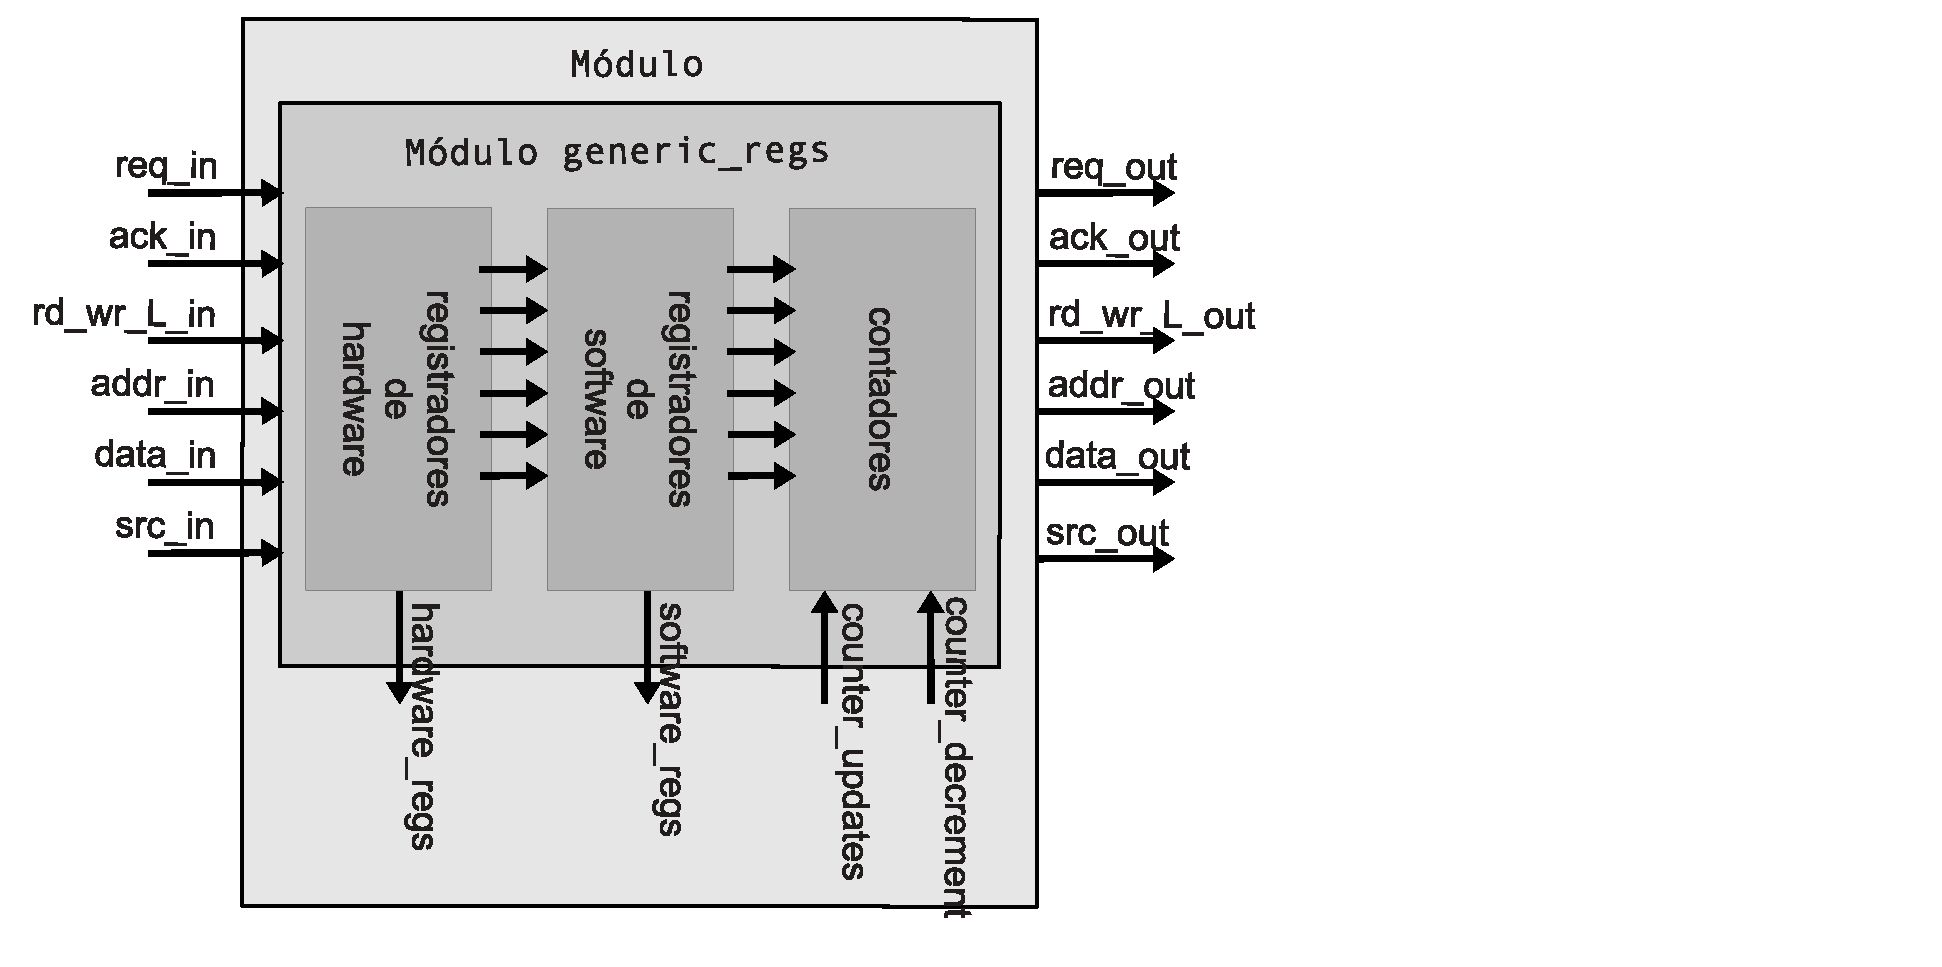
\includegraphics[scale=0.6,angle=0]{figures/modulos/genregister.eps}
\caption{Módulo \ssf{generic\_regs} e barramento de registradores.}
\label{fig:impl.regs.bus}
\end{figure}

O \ssf{nf\_register\_gen} gera blocos para armazenamento de
registradores automaticamente.  Para projetos com requisitos
específicos, é possível controlar o endereço base dos registradores
de cada módulo no arquivo XML de configuração do projeto.  Por
exemplo, para posicionar os registradores do nosso \emph{firewall}
no endereço \ssf{0x02000400} basta utilizar a configuração a seguir.

\begin{minted}{xml}
<!-- netfpga/projects/firewall/include/project.xml -->
<nf:memalloc layout="reference">
    <nf:group name="udp">
        <nf:instance name="firewall" base="0x02000400"/>
        ...
    </nf:group>
    ...
</nf:memalloc>
\end{minted}

Nosso \emph{firewall} lê as portas que devem ser filtradas da
memória SRAM (sexto estágio).  Esta decisão de projeto é didática,
para exemplificar a utilização da memória SRAM.  Num projeto real,
as portas poderiam ser lidas diretamente dos registradores
\ssf{dport0}, \ssf{dport1}, \ssf{dport2}, \ssf{dport3}.  Para que
possa ler as portas TCP bloqueadas da memória SRAM, nosso
\emph{firewall} precisa também gravar esta informação na memória.
Isto é realizado gravando os registradores na memória usando o
módulo \ssf{sram\_arbiter}.  Para detectar se as portas bloqueadas
foram modificadas, verificamos se o uma requisição de registrador
foi atendida (\ssf{reg\_ack\_out}) e se o endereço da requisição
pertence ao nosso módulo (\ssf{tag\_hit} e \ssf{addr\_good}).  Para
verificar se o endereço da requisição pertence ao nosso módulo,
utilizamos as constantes geradas pelo \ssf{nf\_register\_gen}.

\begin{verilogcode}
   always @(*) begin
      wr_data_next <= {dport3[15:0], dport2[15:0],
                       dport1[15:0], dport0[15:0]};
      wr_addr_next <= SRAM_PORTS_ADDR;
      if(tag_hit && addr_good && reg_ack_out)
         wr_req_next <= 1;
      else
         wr_req_next <= 0;
   end
   assign addr_block = reg_addr_out[`UDP_REG_ADDR_WIDTH-1:
                                    `FIREWALL_REG_ADDR_WIDTH];
   assign tag_hit = `FIREWALL_BLOCK_ADDR == addr_block;
   assign addr_good = reg_addr_out[`FIREWALL_REG_ADDR_WIDTH-1:0] >= 
    `FIREWALL_DPORT0 && reg_addr_out[`FIREWALL_REG_ADDR_WIDTH] <= 
    `FIREWALL_DPORT3;
\end{verilogcode}

As linhas \ssf{addr\_block} são construídas a partir do endereço da
requisição e contém o identificador do bloco de registradores (linha
10).  O identificador do bloco de registradores pode ser utilizado
para verificar se o registrador pertence ao nosso módulo (linha 12).
Por último, a linha \ssf{addr\_good} indica se o registrador escrito
é um dos registradores que armazena as portas TCP bloqueadas (linha
13).


\subsection{Sistema de testes}
\label{sec:impl.test}

O \emph{software} da NetFPGA tem um \emph{framework} que projetos
podem utilizar para facilitar e automatizar o desenvolvimento e
execução de testes.

O programa \ssf{nf\_test.py} executa testes armazenados dentro do
subdiretório \ssf{test} no diretório do projeto apontado pela
variável de ambiente \ssf{NF\_DESIGN\_DIR}. O nome de cada teste
deve seguir um formato específico, indicando se é um teste de
simulação (\ssf{sim}), um teste do \emph{hardware} sintetizado
(\ssf{hw}) ou ambos (\ssf{both}); o componente sendo testado
(\ssf{major}); e o teste específico (\ssf{minor}).  Por exemplo, o
comando abaixo irá executar o teste em
\ssf{projects/firewall/test/sim\_firewall\_tcp}.

\begin{minted}{bash}
# inside the NetFPGA root directory
export NF_DESIGN_DIR=$(pwd)/projects/firewall
bin/nf_test.py --isim --major firewall --minor tcp sim
\end{minted}

O \ssf{nf\_test.py} chama o \emph{script} \ssf{run.py} dentro do
diretório do teste.  Os \emph{scripts} \ssf{run.py} podem utilizar
funções da biblioteca de testes da NetFPGA.\footnote{As bibliotecas
do \emph{framework} de testes ficam no diretório
\sssf{lib/python/NFTest}.  As funções relativas a manipulação de
pacotes estão em \sssf{PacketLib.py} e as funções relativas à
comunicação via interface PCI estão em \sssf{NFTestLib.py}.} A
biblioteca possui funções que permitem construir pacotes de rede
usando a biblioteca Scapy\footnote{Scapy, disponível em
\sssf{www.secdev.org/projects/scapy/}.} disponível no Python.  A
biblioteca injeta os pacotes gerados interfaceando com o simulador
ou com o \emph{hardware} dependendo do tipo de teste sendo
realizado.  A biblioteca também permite verificar se pacotes foram
transmitidos ou não.  No teste \ssf{sim\_firewall\_tcp} criamos
pacotes TCP com diferentes portas de destino e depois verificamos se
os pacotes cujas portas não estão bloqueadas foram encaminhados.
Caso pacotes sejam erroneamente encaminhados ou descartados, o teste
resultará em erro.

\begin{minted}{python}
   # projects/firewall/test/sim_firewall_tcp/run.py
   eth_hdr = scapy.Ether(dst=DA, src=SA)
   ip_hdr = scapy.IP(dst=DST, src=SRC)
   tcp_hdr = scapy.TCP(dport=random.choice(POSSIBLE_PORTS), sport=SPORT)
   ...
   pkt = eth_hdr/ip_hdr/tcp_hdr/payload
   nftest_send_phy('nf2c0', pkt)
   if(pkt.dport not in BLOCKED_PORTS):
      ...
      nftest_expect_dma('nf2c0', pkt)
\end{minted}

A biblioteca também possui funções que permitem escrever e ler
valores de registradores e da memória SRAM.  Para tornar o teste
\ssf{sim\_firewall\_tcp} interessante, utilizamos as funções da
biblioteca para configurar as portas que devem ser filtradas, bem
como verificar se a configuração foi escrita no registrador.  Note
que o módulo Python \ssf{reg\_defines} é gerado pelo
\ssf{nf\_register\_gen}.

\begin{minted}{python}
# projects/firewall/test/sim_firewall_tcp/run.py
nftest_regwrite(reg_defines.FIREWALL_DPORT0_REG(),
                BLOCKED_PORTS[0])
nftest_regread_expect(reg_defines.FIREWALL_DPORT0_REG(),
                      BLOCKED_PORTS[0])
\end{minted}

Podemos também verificar se as portas foram escritas na primeira
linha de memória de onde nossa máquina de estados lê as portas que
devem ser bloqueadas.  Adicionamos um pequeno atraso no
\emph{script} de teste para dar tempo para os dados serem gravados
na memória.  A manipulação dos bits é necessária devido ao formato
no qual as portas são gravadas na memória SRAM.

\begin{minted}{python}
simReg.regDelay(1000)
nftest_regread_expect(reg_defines.SRAM_BASE_ADDR(),
                      BLOCKED_PORTS[2]<<16 | BLOCKED_PORTS[3])
\end{minted}

A saída do \ssf{nf\_test.py} contém o tempo de simulação e as
mensagens escritas.  Estas mensagens podem ser geradas de dentro do
código Verilog usando as diretivas \ssf{\$display}.  As funções
disponibilizadas pelo sistema de testes em Python geram mensagens
indicando qual operação será realizada e o seu resultado. Por
exemplo, as asserções de leitura sobre endereços definidos nos
arquivos de cabeçalho normalmente produzem a mensagem \emph{``Good:
PCI read of addr X returned data Y as expected''} quando o resultado
está correto. O final da saída indica se todas as verificações do
teste passaram através da mensagem \emph{``Test X passed!''} e
vice-versa.






\newpage
\section{Trabalhos relacionados}
\label{sec:related}

Apresentaremos nesta seção, uma revisão de trabalhos relacionados
com a NetFPGA. Destaca-se que desde 2006, quando o projeto ganhou
maior popularidade, já foram publicados mais de 226 artigos
acadêmicos envolvendo a NetFPGA como parte de pesquisa cientifica em
redes de computadores ou sistemas distribuídos, e existe uma extensa
listagem de mais de 40 projetos com código aberto, tanto nas versões
de NetFPGA 1G quanto nas versões mais recentes da NetFPGA 10G, CML e
SUME. Nesta breve revisão destacaremos as contribuições mais
importantes.

\subsection{Artigos Acadêmicos}

A plataforma NetFPGA teve sua origem em um curso de pós-graduação
CS344 de Stanford~\cite{4589059}, onde os alunos trabalhavam em um
projeto para criar um roteador tanto com componentes em
\textit{hardware} e em \textit{software} em oito semanas. Parte da
motivação deste curso, veio da experiencia na indústria de alguns
dos professores como Nick McKweon (um dos arquitetos do roteador
Cisco GSR 12000). Na indústria, destacava-se que os estagiários e
recém-contratados, ou entendiam bem de \textit{hardware} ou
entendiam bem de \textit{software}, mas não os dois ou sua
integração. Adicionalmente ao ensino, a construção de um sistema
aberto como a NetFPGA também propiciou um ambiente para pesquisa de
alta qualidade em redes~\cite{Naous:2008:NRR:1397718.1397720}.

Dentre os primeiros projetos, os alunos do curso contribuíram com
roteadores e comutadores de referência, bem como sistemas de
monitoração de \emph{buffers} e geradores de pacotes altamente
precisos~\cite{5290917}. Em 2008, auxiliado pela popularidade da
tecnologia OpenFlow, foi desenvolvido uma implementação de um
comutador OpenFlow em NetFPGA~\cite{Naous:2008:IOS:1477942.1477944}.
Esta foi uma das primeiras soluções de comutador OpenFlow flexíveis,
de alta velocidade e baratas para pesquisa em SDN. E posteriormente,
tornou a NetFPGA um elemento presente em ambientes de produção de
diversas plataformas de experimentação OpenFlow internacionais como
GENI, KOREN e o FIBRE~\cite{1649119}.

Os projetos de desenvolvimento foram ganhando mais sofisticação
dentro de vários \textit{Workshops} de Desenvolvimento específicos
em NetFPGA, tanto em Stanford quanto em Cambridge-UK, e em outras
partes do mundo.  Esses \textit{Workshops} popularizaram trabalhos
técnicos em várias áreas, que faziam uso da plataforma. Adicionando,
por exemplo, projetos em suporte a \textit{drivers} para Windows ou
a implementação de protótipo de envio de sinal de rádio GNURadio
empacotado em pacotes IP~\cite{airnetfpga}.

Outros trabalhos oriundos dos \textit{Workshops} concentram as
publicações de trabalhos relacionados nos anos de 2009 e 2010. A
partir de 2011, a quantidade de trabalhos que usa ou avança o
progresso da NetFPGA aumenta consideravelmente, diversificando sua
atuação em diversas publicações especializadas em redes ou FPGAs em
congressos da ACM e IEEE, e portanto não mais restrito aos
\textit{Workshops}. Um pequeno resumo de alguns desses projetos
segue, ordenados cronologicamente:

\begin{itemize}

\item \textit{Fast Reroute and Multipath}~\cite{multipath}: trata-se
de um projeto onde a partir do roteador de referência foi adicionado
a possibilidade de recuperação de rotas por \emph{hardware}, em caso
de falha. E uma implementação do protocolo ECMP (\emph{Equal Cost
Multipath}) para realizar o balanceamento de carga de fluxos entre
as interfaces da NetFPGA.

\item \textit{NetThreads -- Programming NetFPGA with Threaded
Software}~\cite{6645624}: A ideia consiste na implementação de uma
arquitetura soft-core baseada em NetFPGA multiprocessada e
\emph{multithreaded}, para que aplicações de rede que têm
paralelismo inerente possam se beneficiar e acelerar aplicações
paralelas, com melhoria no compartilhamento dos dados e na
sincronização no nível físico.

\item \textit{DFA-based Regular Expression Matching}~\cite{dfa}:
Esse projeto trata de capturar através de regras do aplicativo
\textit{Snort} e usando expressões regulares transformadas em
autômatos determinísticos finitos (DFA) em \textit{hardware}. Desse
modo, determinados fluxos são capturados baseados em classificação
de cabeçalhos de pacotes. Os estados são manipulados na memória da
placa e também fora da mesma e existe um rastreamento da transição
de estados no chip para verificar se determinado pacote casa com uma
regra complexa.

\item \textit{OpenPipes -- Prototyping High-speed Networking
Systems}~\cite{openpipes}: Trata-se de uma plataforma de criação de
``sistemas distribuídos'' em \textit{hardware}, onde cada componente
pode ficar em um computador separado, interligado em rede. Esses
componentes se comportam como tubos (\textit{pipes}), tornando a
criação modular e simples, de sistemas baseados em \textit{hardware}
escaláveis. Na demonstração, os autores usam módulos de
processamento de vídeo embarcados na placa, como suavização de
imagem, conversão para tons de cinza e inversão de cores, e
separados em diferentes máquinas em rede, onde a execução
distribuída é feita com a ajuda da NetFPGA integrando os dados.

\item \textit{PortLand -- A Scalable Fault-Tolerant Layer 2 Data
Center Network
Fabric}~\cite{NiranjanMysore:2009:PSF:1592568.1592575}: Este
trabalho apresenta a concepção de uma rede de centro de
processamento de dados totalmente baseada em camada de enlace, com
tolerância a falhas e alto desempenho. Isso é obtido pelo reuso do
endereçamento MAC de maneira a permitir a migração de máquinas
virtuais intra-rack e inter-rack, e a manutenção de sua
conectividade IP. A avaliação do projeto, em alta velocidade, contou
com um conjunto de cerca de 40 NetFPGAs. Esse foi um dos primeiros
trabalhos a usarem a NetFPGA como apoio à validação experimental em
pesquisa em redes de alta velocidade.

\item \textit{BCube: A High Performance, Server-centric Network
Architecture for Modular Data
Centers}~\cite{Guo:2009:BHP:1592568.1592577}: Outro artigo na mesma
linha do Portland, focado em uma nova arquitetura de rede para
centros de processamento de dados. A ideia é um tipo de rede
centrada em interligação de servidores, sem apresentar equipamentos
de rede como comutadores ou roteadores. Os servidores agem como
encaminhadores de tráfego, além de pontos finais de comunicação.
Outras características importantes são tolerância a falhas e
balanceamento de carga. Destaca-se que a implementação da prova de
conceito foi toda feita em NetFPGA.

\item \textit{Using NetFPGA to Offload Linux Netfilter
Firewall}~\cite{netfilter}: O \emph{framework} Netfilter está
localizado na camada IP do Linux e é caracterizado por uma série de
ganchos (pontos de entrada) que permitem interceptar e manipular
pacotes que atravessam a camada IP. Normalmente, ferramentas como o
\ssf{iptables} permitem a comunicação direta com o Netfilter por
meio de soquetes Netlink, de modo a realizar chamadas de sistema nos
pontos dentro do \emph{kernel} e manipular ou descartar pacotes. O
projeto modifica o \ssf{iptables} e descarrega algumas regras
Netfilter direto para o \emph{hardware} por meio da NetFPGA,
liberando a CPU para outras atividades.

\item \textit{A Randomized Scheme for IP Lookup at Wire Speed on
NetFPGA}~\cite{5502019}: Os tempos de busca em uma tabela de
encaminhamento (chamados de \textit{lookups}) precisam ser em geral
muito baixos, embora o tamanho das tabelas na Internet só cresça.
Nesse sentido, os autores deste trabalho apresentam um novo esquema
de busca de endereços usando a NetFPGA, que faz uso de buscas em
paralelo feitas com funções de \textit{hash} perfeitas. Essas
funções trabalham com uma estrutura de dados de rápido acesso e
bastante compactas chamadas de \textit{Blooming Trees}.

\item \textit{BORPH: An Operating System for the NetFPGA
Platform}~\cite{borph}: O artigo BORPH apresenta o conceito de um
sistema operacional projetado para trabalhar com computadores
reconfiguráveis baseados em FPGA. A prova de conceito é feita por um
conjunto de extensões do Linux. Dado a facilidade de reconfiguração
pelo barramento PCI que a NetFPGA habilita, o sistema foca em prover
abstrações UNIX como arquivos, de modo a ter acesso direto a
recursos de registradores e processamento da NetFPGA bem como
reconfigurar partes do \emph{hardware} sob demanda.

\item \textit{The Click2NetFPGA Toolchain}~\cite{180848}: Nesse
trabalho, a ideia é facilitar a aceleração promovida pela NetFPGA na
área de aplicações em rede, através do uso de um sintetizador de
alto nível. Em resumo, a partir de uma descrição de um roteador com
linguagem de domínio e componentes básicos em C++ usados no
\textit{Click Modular Router}. O artigo se propõe a transformar
automaticamente código existente dentro desse domínio específico em
um projeto de \textit{hardware} funcional. A cadeia de ferramentas
faz uso de LLVM, como linguagem de abstração intermediária, depois
uma optimização usando uma técnica chamada AHIR que permite, a
partir de uma estrutura bem definida LLVM, produzir o código VHDL
para a NetFPGA.

\end{itemize}

Com essa revisão de trabalhos relacionados podemos verificar a ampla
cobertura e exuberante quantidade de desenvolvimento que a
plataforma NetFPGA tem atraído. No que segue nesta seção, daremos
destaque em maior profundidade a dois projetos de alto impacto para
a realização de pesquisas em redes: a implementação do comutador
OpenFlow na NetFPGA e o \emph{Software} Testador de Redes OSNT, que
permite geração de tráfego para testes de desempenho de alta
precisão.

\subsection{Implementação de OpenFlow na NetFPGA}

Nesta seção, descreveremos a implementação do OpenFlow em uma placa
NetFPGA~\cite{Naous:2008:IOS:1477942.1477944}. A princípio é preciso
observar que boa parte da complexidade do comutador OpenFlow é
oriunda de outros elementos NetFPGA de referência como partes da
placa de rede de quatro portas, comutador e roteador IPv4. A
implementação possui duas partes relevantes: o \emph{software} de
gerenciamento, lado que trata as mensagens do protocolo OpenFlow
1.0, e a aceleração da tabela de fluxos (\textit{flow table}) em
\emph{hardware}.

O \emph{software} de gerenciamento do comutador OpenFlow é baseado
na implementação de referência de comutadores OpenFlow de Stanford.
Trata-se de um \emph{software} aberto para Linux que implementa todo
o comportamento de um comutador OpenFlow. Este software de
referência pode ser dividido em duas seções: o programa que executa
em espaço de usuário e o módulo do \emph{kernel}.

O processo que executa em espaço de usuário se comunica por soquete
com o controlador OpenFlow usando SSL para criptografar a
comunicação.  O processo coordena o envio das mensagens do comutador
para o controlador e vice-versa, tratando chegadas de novos fluxos
ou atualizações do estado dos enlaces do comutador. As mensagens de
controle permitem adicionar ou remover entradas da tabela de fluxos
e são implementadas através de chamadas de sistema \ssf{ioctl} entre
o programa que executa em espaço de usuário e o módulo do
\emph{kernel}.

O módulo do \emph{kernel} é responsável por manter as tabelas de fluxo,
processar pacotes, encaminhar, reescrever cabeçalhos e atualizar
estatísticas.  Por definição, o módulo do \emph{kernel} do comutador
OpenFlow de referência cria a tabela de fluxo em \emph{software}, e vai
testando as cadeias de regras por um casamento sequencialmente. A
prioridade é dada para a primeira regra que casar dentro da cadeia.

Ainda no módulo do \emph{kernel} é possível estender a tabela de
fluxos para fazer uso de processamento em \textit{hardware} na
NetFPGA.  Os pacotes que chegam na NetFPGA fazem acesso rápido as
entradas da tabela de fluxo armazenadas na NetFPGA e encaminha os
pacotes com casamento na mesma taxa dos enlaces (por exemplo,
1\,Gbps por porta). Por sua vez, pacotes que não casem com regras de
fluxo existentes (por exemplo, fluxos novos) são enviados para o
módulo do \emph{kernel} do OpenFlow, onde serão tratados.  Pacotes
sem casamento podem chegar ao programa em espaço do usuário, que irá
gerar um evento \ssf{pkt\_in} e enviá-lo ao controlador.

\begin{figure}[h]
\centering
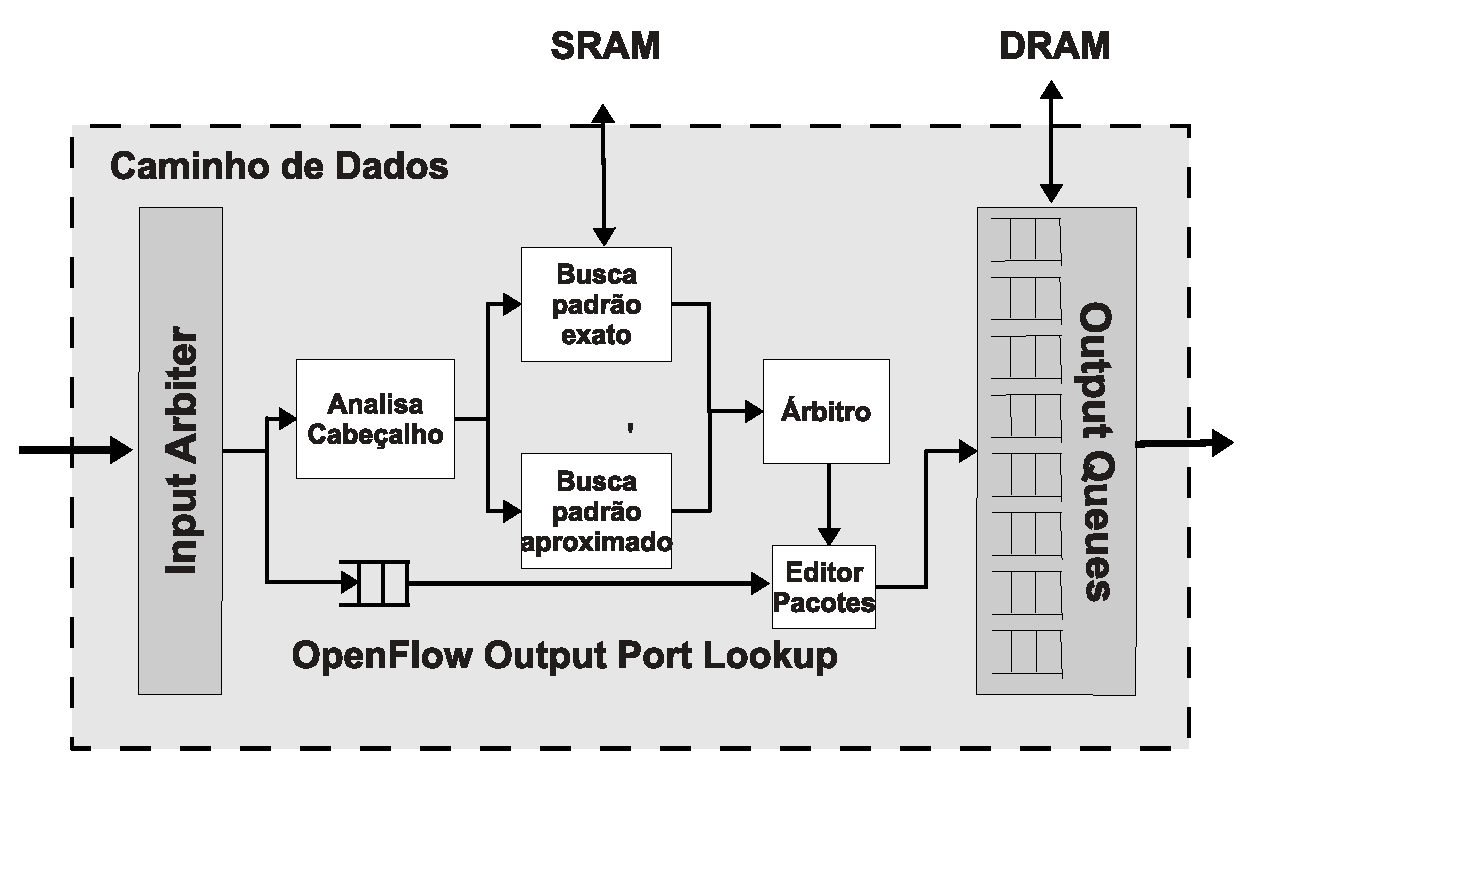
\includegraphics[scale=0.4]{figures/netfpga-rev/nfopenflow.eps}
\caption{Componentes do comutador OpenFlow NetFPGA.}
\label{fig:nfopenflow}
\end{figure}

Ilustramos o módulo \ssf{output\_port\_lookup} do comutador OpenFlow
na \figstr~\ref{fig:nfopenflow}.  Primeiro ele concatena cerca de
dez campos num cabeçalho de fluxo (\emph{flow header}), e envia esse
cabeçalho para busca nas tabelas de roteamento. A busca é feita em
paralelo utilizando uma combinação de memórias ternárias (TCAMs) no
FPGA e memória SRAM para suportar tanto a possibilidade de
``coringas'' (prefixos) na TCAM quanto um grande número de entradas
exatas de fluxos na SRAM.

Essa busca de entradas exatas utiliza de uma função de \emph{hash}
do cabeçalho de fluxo para indexar a SRAM, reduzindo a necessidades
de memória e colisões. Após o casamento de uma regra, o módulo
possui uma fase de tomada de ações, através de um árbitro.  O
árbitro pode editar campos do pacote antes de encaminhá-lo para as
filas de saída. Essa fase de ações está associada à sequência dos
casamentos, com uma ação definida para cada regra com casamento.

\subsection{OSNT: Open Source Network Tester}

O segundo projeto que descreveremos em maior detalhe é a
implementação de um testador de rede usando a
NetFPGA-10G~\cite{shahbaz2013arch}. A solução é código aberto e de
alto desempenho operando a 10Gbps, custa para um pesquisador pouco
menos de 2 mil dólares, sendo que equipamento equivalente em
\textit{hardware} na indústria especializada custa 25 mil dólares. A
placa usa um FPGA mais recente e tem a habilidade de trabalhar com
múltiplos \textit{pipelines} de processamento. Entre esses,
destacamos somente o subsistema de geração de tráfego, na figura
\ref{fig:osnt1}. Existem outros subsistemas, por exemplo para
encapsulamento de pacotes para virtualização e de monitoração
passiva e precisa de tráfego.

\begin{figure}[h]
\centering
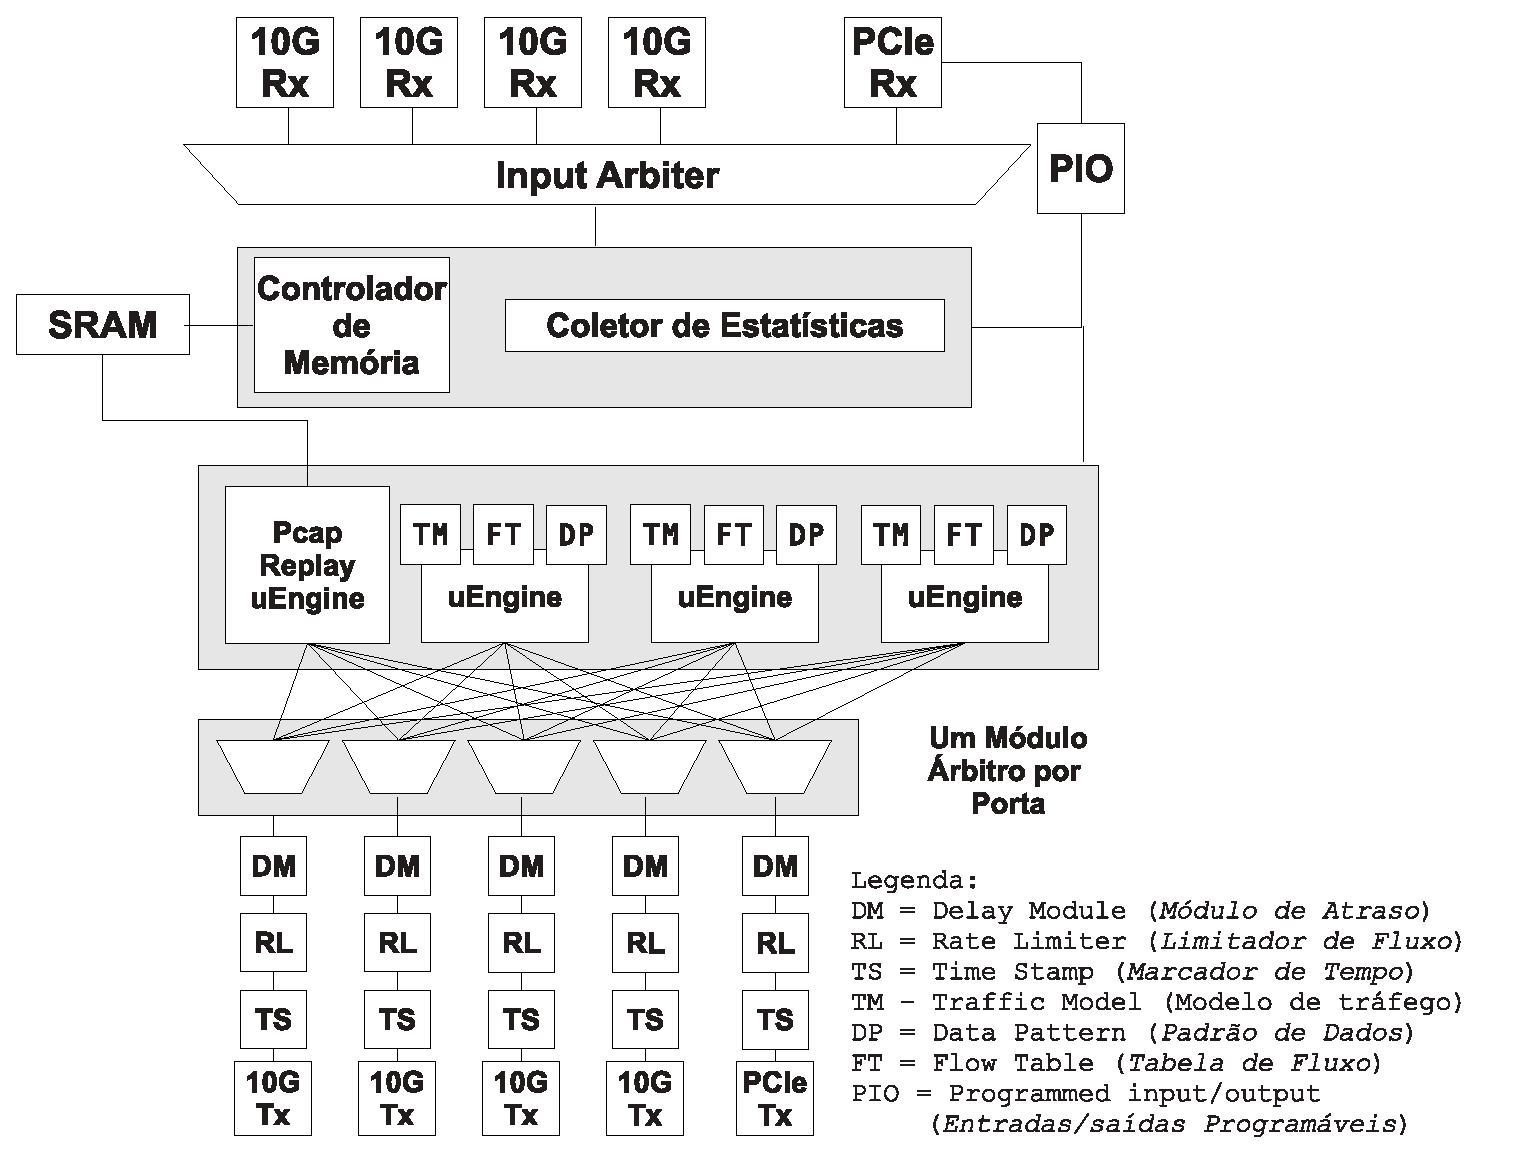
\includegraphics[scale=0.5]{figures/netfpga-rev/osnt1.eps}
\caption{\emph{Pipeline} de Geração de Tráfego da OSNT.}
\label{fig:osnt1}
\end{figure}

O \textit{pipeline} gerador de tráfego gera pacotes e analisa
estatísticas. O gerador de tráfego consiste de pequenos
\textit{micro-engines}, cada qual gera tráfego de acordo com um
modelo de tráfego (TM, \emph{traffic model}) configurado, uma lista
de valores para os cabeçalhos dos fluxos (FT) e certos padrões de
como gerar o tamanho do pacote, sua taxa e os atrasos entre pacotes
(DP).  Adicionalmente é possível gerar tráfego a partir de um
\textit{trace} \ssf{pcap} (via \ssf{tcpdump}). Após essa fase de
moldagem dos fluxos, existem cinco unidades funcionais para efetivar
a transmissão: o árbitro seleciona os pacotes e os encaminha quando
for o tempo correto de envio.  Depois, o módulo de atraso (DM)
controla o atraso, o módulo de limitação de taxa (RL) limita cada
fluxo (implementando algoritmo equivalente a um \emph{token
bucket}), o módulo de marcação de tempo (TS) computa quando o pacote
foi transmitido e por último o pacote é enviado.

\subsection{Futuro da NetFPGA: Projetos NetFPGA-10G, 10G-CML e 10G-SUME}

Redes de centros de processamento de dados vêm motivando a adoção de
sistemas de rede mais rápidos. As velocidades oferecidas pela
NetFPGA 1\,Gbps, embora interessantes do ponto de vista de ensino,
são bastante defasadas em termos de velocidade para pesquisa na área
de centros de processamento de dados.

Nesse sentido, o projeto NetFPGA, ao longo dos anos vem colocado a
disposição placas de 10\,Gbps, a mais recente com capacidade de I/O
de 100\,Gbps~\cite{6866035}. Dessa forma, o projeto fica atualizado
com relação a uma nova geração de dispositivos de alta velocidade.
Ou seja, permite testar novas ideias em escala compatível com
ambientes de centros de processamento de dados, em empresas como
Localweb, UOL, ou Facebook. A NetFPGA 1G era uma placa de baixo
custo projetada usando um FPGA Xilinx Virtex-II Pro 50. Por sua vez,
em 2010, foi lançada a placa NetFPGA 10G, que expandia a plataforma
original para trabalhar com transmissões até 40\,Gbps sendo 10\,Gbps
por interface, com interface PCIe Gen~1, e baseado no FPGA Xilinx
Virtex-5 FPGA.

Posteriormente, a placa 10G-CML desenvolvida pela empresa
especializada em segurança cibernética CML (\textit{Computer
Measurement Lab}), atualizou o FPGA para o Xilinx Kintex-7 325T, e o
I/O é baseado no adaptador PCIe x4 Gen~2, com alto desempenho. A
última linha de placa que surgiu em 2014 é a 10G-SUME~\cite{6866035}
conforme mostra a figura \ref{fig:sume}.

\begin{figure}[h]
\centering
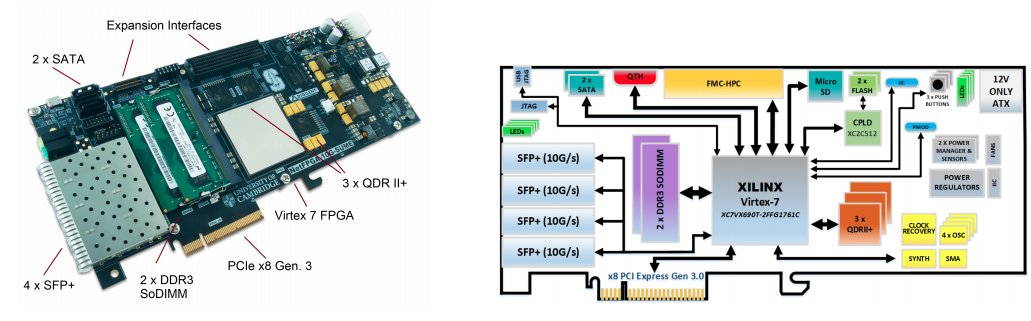
\includegraphics[scale=0.4]{figures/netfpga-rev/sume.png}
\caption{Foto e Arquitetura da Placa SUME.}
\label{fig:sume}
\end{figure}

A placa NetFPGA SUME é uma placa de custo mais elevado, porém o
preço é subsidiado para pesquisa acadêmica. Além disso ela possui
capacidade de I/O aumentada com operações de até 100\,Gbps através
do adaptador PCIe x8 Gen~3 e também incorpora um  FPGA mais poderoso
que é o Xilinx’s Virtex-7 690T. Para demonstrar as capacidades da
placa SUME, os pesquisadores utilizaram três placas para montar um
comutador OpenFlow com 12 interfaces de 10\,Gbps interligadas por um
\emph{backplane} não-blocante de 300\,Gbps.

Enfim, o futuro da NetFPGA parece bastante promissor em termos de
avanços na área de alto desempenho. O \textit{software} de todos os
projetos desenvolvido  está disponível no GitHub e é licenciado como
\emph{software} livre sob a licença LGPL 2.1, o que permite ser
utilizado em projetos comerciais.


\section{Conclusões e perspectivas}

Neste trabalho apresentamos a plataforma NetFPGA através da demonstração
passo-a-passo do desenvolvimento de uma aplicação real.  A aplicação
consiste de um \emph{firewall} para filtragem de pacotes em
\emph{hardware}. Os conceitos básicos da arquitetura da NetFPGA foram
discutidos. Mostramos os principais componentes de \emph{hardware} e
\emph{software}. Os aplicativos de referência como placa de rede,
comutador e roteador foram discutidos, além dos módulos de interação
\emph{hardware-software} como a interface de registradores e o
controlador de memória.

Dado o seu potencial no processamento de pacotes, consideramos que a
NetFPGA possui um grande potencial no desenvolvimento de novos projetos
de pesquisa, seja permitindo prover novas funcionalidades no plano de
dados, seja como ferramenta para o desenvolvimento de novos padrões e
protocolos de comunicação, seja no desenvolvimento de novos protótipos
de pesquisa.  Certamente, a NetFPGA ajudará no desenvolvimento de
trabalhos interessantes e com grande potencial na área de redes de
computadores.


\section*{Apêndice A: Diretivas de programação}
\label{sec.impl.apendice}

Neste material adotamos algumas convenções para facilitar o
entendimento, listadas a seguir. Alguns dos exemplos citados são
recomendações de boas técnicas comuns em linguagens de programação,
enquanto outras são necessárias para que o hardware resultante alcance o
comportamento desejado do projeto.\footnote{As recomendações foram
extraídas e adaptadas de
\sssf{http://www.xilinx.com/itp/xilinx10/books/docs/sim/sim.pdf} e
\sssf{https://github.com/NetFPGA/netfpga/wiki/VerilogCodingGuidelines}.}

\begin{itemize}

\item Use constantes e parâmetros para conferir legibilidade ao código.
Defina constantes em letra \ssf{MAIÚSCULA}.

\item Trechos do código que fazem asserções, monitoram ou imprimem
valores de variáveis para teste do projeto devem estar posicionadas
entre as diretivas \ssf{synthesis translate\_off} e \ssf{synthesis
translate\_on}. Estes trechos são executados na simulação, mas são
ignorados pelo sintetizador na criação do \emph{bitfile} do projeto.

\item Em circuitos sequenciais utilize somente atribuições não-blocantes
(\ssf{<=}) dessa forma todas as atribuições dentro do bloco (geralmente
\ssf{always}) são avaliadas primeiro e depois realizadas na simulação e
permitem ao sintetizador inferir o circuito síncrono. No exemplo a
seguir todas as atribuições são sincronizadas com o sinal de relógio e
recebem os valores anteriores dos sinais, ou seja, a sequência não
importa:

\begin{verilogcode}
always @(posedge clk) begin
    B <= A;
    C <= B;
    D <= C;
end
\end{verilogcode}

\item Em circuitos combinacionais certifique-se de preencher a lista de
sensibilidade com todas as variáveis de interesse ou usar \ssf{always
@(*)}. Nesses circuitos qualquer alteração em alguma das variáveis na
lista forçam a reexecução do bloco (em geral \ssf{always} ou
\ssf{assign}) imediatamente. Certifique-se também de somente utilizar
atribuições blocantes (\ssf{=}) para que o sintetizador infira um
circuito assíncrono. O parâmetro \ssf{@(*)} é um recurso do Verilog que
preenche automaticamente a lista de sensibilidade com todos os valores
atribuídos dentro do bloco. No exemplo a seguir, as variáveis B, C e D
recebem o valor de A:

\begin{verilogcode}
always @(*) begin
    B = A;
    C = B;
    D = C;
end
\end{verilogcode}

\item Atribua todas as variáveis em todos os estados possíveis do seu
projeto. Este erro ocorre geralmente em expressões condicionais \ssf{if}
sem a cláusula \ssf{else} ou blocos \ssf{case}. No exemplo abaixo,
\ssf{cnt\_nxt} recebe o valor atual de \ssf{cnt} por padrão, para evitar
que ele deixe de ser atribuído se algum estado não requerer sua
atualização, e \ssf{state\_nxt} é atribuído em todos os estados. 

\item Em lógicas de controle é recomendado criar circuitos
combinatoriais que recebam os valores do próximo estado. Os valores do
próximo estado devem ser guardados em registradores em circuitos
síncronos com a borda do relógio:

\begin{verilogcode}
always @(*) begin
    cnt_nxt = cnt;  
    case(state)
        INCREMENTA: begin 
            if(cnt == 99)
                state_nxt = RESETA;
            else begin
                cnt_nxt = cnt+'h1;
                state_nxt = INCREMENTA;
        end    
        RESETA: begin 
            cnt_nxt = 'h0;
            state_nxt = INCREMENTA;
        end
        DEFAULT: begin
            state_nxt = RESETA;
        end
    endcase
end

always @(posedge clk) begin
    if(reset) begin
        cnt <= 0;
        state <= INCREMENTA;
    end
    else begin
        cnt <= cnt_nxt;
        state <= state_nxt;
    end
end
\end{verilogcode}
%\end{listing}

Nesse exemplo, o circuito combinacional calcula os valores de
\ssf{state} e \ssf{cnt} que serão atualizados na próxima borda de subida
do sinal do relógio pelo circuito sequencial.

\item Não utilize atribuições com atrasos pois são normalmente ignoradas
pelas ferramentas de síntese, o que pode resultar num comportamento
inesperado do projeto.

\begin{verilogcode}
assign #10 Q = 0; // do not use
\end{verilogcode}

\item Utilize blocos \ssf{generate} para gerar várias instâncias de
módulos ou blocos de código. Na \secstr~\ref{sec:impl.mem} utilizamos
\ssf{generate} para criar o vetor com os bits de paridade dos dados a
serem gravados na memória;

\item Outras dicas podem ser encontradas nas páginas Web mencionadas e
livros especializados.

\end{itemize}





\begin{comment}
\mr{movido da introdução}
\pg{O código abaixo escreve zeros em todos os endereços da memoria}
\begin{verbatim}
module reseta_sram #(
		parameter SRAM_DATA_WIDTH = 72,
		parameter SRAM_ADDR_WIDTH = 19
)
(
    output reg [SRAM_DATA_WIDTH-1:0] 	sram_data,
    output reg [SRAM_ADDR_WIDTH-1:0] 	sram_addr,
    output reg [7:0] 					sram_bw,
    output reg 							sram_we,
    output reg 							sram_tri_en,
	input  				    			clk,
	input								reset
    );

	reg									sram_tri_en_1, sram_tri_en_2;
	reg	[SRAM_DATA_WIDTH-1:0]	sram_data_1, sram_data_2;
	   
always @(posedge clk) begin
    if(reset) begin
        sram_addr <= 'h0;
        sram_data_2 <= 'h0;
        sram_bw <= 'h00; 
        sram_we <= 1'b0;
        sram_tri_en_2 = 1'b1;
    end
    else if(sram_addr < {SRAM_ADDR_WIDTH{1'b1}}) begin
        sram_addr <= sram_addr+'b1;
        sram_data_2 <= 'h0;
	    sram_bw <= 8'h00;		  
        sram_we <= 1'b0; 
        sram_tri_en_2 = 1'b1;
    end
    else begin
        sram_bw <= 'hff; 
        sram_we <= 1'b1; 
        sram_tri_en <= 1'b0; 
    end
    //estágio 1 do pipeline de escrita
    sram_tri_en_1 <= sram_tri_en_2;
    sram_tri_en <= sram_tri_en_1;
    //estágio 2 do pipeline de escrita
    sram_data_1 <= sram_data_2;
    sram_data <= sram_data_1;
end
endmodule

\end{verbatim}

Um arquivo de testes é necessário para visualizar o correto funcionamento:
\begin{verbatim}
module uut_reseta_sram #(

    parameter 	PERIOD = 10,
	parameter	SRAM_DATA_WIDTH = 72,
	parameter	SRAM_ADDR_WIDTH = 5
);
	// Inputs
	reg clk;
	reg reset;

	// Outputs
	wire [SRAM_DATA_WIDTH-1:0] 	sram_data;
	wire [SRAM_ADDR_WIDTH-1:0] 	sram_addr;
	wire [7:0] 							sram_bw;
	wire 									sram_we;
	wire 									sram_tri_en;
	
	reg [SRAM_DATA_WIDTH-1:0]		memoria [0:(1<<SRAM_ADDR_WIDTH)-1];
	integer 		idx;

	// Instantiate the Unit Under Test (UUT)
	reseta_sram  #(
	    .SRAM_DATA_WIDTH(SRAM_DATA_WIDTH),
	    .SRAM_ADDR_WIDTH(SRAM_ADDR_WIDTH)
    ) uut (
        .sram_data(sram_data),
        .sram_addr(sram_addr),
        .sram_bw(sram_bw),
        .sram_we(sram_we), 
        .sram_tri_en(sram_tri_en),
        .clk(clk),
        .reset(reset)
    );

	initial begin
        $dumpfile("sram.vcd");
        for(idx=0;idx<(1<<SRAM_ADDR_WIDTH);idx=idx+1)
            $dumpvars(0,memoria[idx]);
        $dumpvars(0,uut_reseta_sram);
        clk = 0;
        reset = 0;
        #5 reset = 1;
        #30 reset = 0;
        #1000 $finish;
    end

    always begin
        clk = 1'b0;
        #(PERIOD/2) clk = 1'b1;
        #(PERIOD/2);
    end  
	
	always @(*) begin
        if(!sram_we && sram_tri_en) begin
            if(sram_bw[0])
                memoria[sram_addr][8:0] <= memoria[sram_addr][8:0];
            else	
                memoria[sram_addr][8:0] <= sram_data[8:0];
            if(sram_bw[1])
                memoria[sram_addr][17:9] <= memoria[sram_addr][17:9];
            else
                memoria[sram_addr][17:9] <= sram_data[17:9];
            if(sram_bw[2])
                memoria[sram_addr][26:18] <= memoria[sram_addr][26:18];
            else
                memoria[sram_addr][26:18] <= sram_data[26:18];
            if(sram_bw[3])
                memoria[sram_addr][35:27] <= memoria[sram_addr][35:27];
            else
                memoria[sram_addr][35:27] <= sram_data[35:27];
            if(sram_bw[4])
                memoria[sram_addr][44:36] <= memoria[sram_addr][44:36];
            else
                memoria[sram_addr][44:36] <= sram_data[44:36];
            if(sram_bw[5])
                memoria[sram_addr][53:45] <= memoria[sram_addr][53:45];
            else
                memoria[sram_addr][53:45] <= sram_data[53:45];
            if(sram_bw[6])
                memoria[sram_addr][63:54] <= memoria[sram_addr][63:54];
            else
                memoria[sram_addr][63:54] <= sram_data[63:54];
            if(sram_bw[7])
                memoria[sram_addr][71:63] <= memoria[sram_addr][71:63];
            else
                memoria[sram_addr][71:63] <= sram_data[71:63];				
        end
    end
endmodule
\end{verbatim}


\pg{O arquivo de testes instancia o módulo para limpar a SRAM e demonstra o resultado da escrita, além de permitir a visualização em forma de onda das mudanças do conteúdo da memória. Essa simulação pode ser gerada, por exemplo, através das ferramentas Icarus Verilog e GTK-Wave que podem ser instaladas pelo yum através de:}

\begin{verbnobox}
sudo yum install iverilog
sudo yum install gtkwave
\end{verbnobox}

O comando a seguir invoca o compilador e gera um arquivo binário para ser executado pelo simulador:
\begin{verbnobox}
iverilog uut_reseta_sram reseta_sram -o srambin
\end{verbnobox}

O simulador gerará um arquivo de saída de nome sram.vcd, conforme definido no comando \$dumpfile:

\begin{verbnobox}
vvp srambin
\end{verbnobox}

Você verá uma mensagem indicando que o arquivo com as formas de onda foi criado:

\begin{verbnobox}
VCD info: dumpfile sram.vcd opened for output.
\end{verbnobox}

Agora invocamos o gtkwave para ler o arquivo gerado com o comportamento das variáveis:

\begin{verbnobox}
gtkwave sram.vcd
\end{verbnobox}

A simulação do projeto em formas de ondas é útil para identificarmos erros no comportamento em módulos isolados ou em conjuntos de módulos que possam ser encapsulados numa interface bem definida, entretanto esta tarefa não é trivial quando o projeto é constituído de dezenas de módulos. A NetFPGA possui enfoque em testes de regressão \pg{citar pagina que explica os testes de regressao}. Ela oferece funcionalidades que permitem testes extensivos sobre o projeto. %, o que normalmente não é trivial para ser feito através das formas de onda devido à dificuldade em rastrear as variáveis internas de todos os módulos instanciados no projeto, ou mesmo de se descrever o comportamento do projeto final a partir delas.
\end{comment}


\newpage
\bibliographystyle{sbc}
\bibliography{ref}

\end{document}
